\documentclass[a4paper,titlepage]{caspset}
\usepackage{pgfpages}
%\usepackage[left=0.1in,right=0.1in,top=0.1in,bottom=0.45in]{geometry}
%\usepackage[frame,center,noinfo]{crop}
%\usepackage{handoutWithNotes}
%\pgfpagesuselayout{4 on 1 with notes}[a4paper,border shrink=5mm]
%\pgfpagesuselayout{4 on 1}[a4paper,border shrink=5mm]
\usepackage{fancyhdr}
% set 1-inch margins in the document
\usepackage[left=0.75in,right=0.75in,top=1.2in,bottom=1in]{geometry}
%\usepackage[left=0.2in,right=0.2in,top=0.5in,bottom=0.5in]{geometry}
\usepackage{lastpage}
% include this if you want to import graphics files with /includegraphics
\usepackage{graphicx}
\usepackage{lastpage}
\usepackage{pdfpages}
\usepackage[toc,page,title,titletoc,header]{appendix}
\usepackage[unicode]{hyperref}
%\newcommand{\chapter}[1]{\begin{center}\large\sffamily{#1}\end{center}}
\usepackage{multicol} 
\usepackage{titlesec}

%%%%%%%%%%%%%%%%%%%%%%%%%%%%%%%%%%%%%%%%%%%%%%%%%%%%%%
\usepackage{xeCJK}
%\usepackage{fontspec}
\setCJKmainfont[BoldFont=simhei.ttf]{simsun.ttf}
\setCJKsansfont{simhei.ttf}
\setCJKmonofont{simfang.ttf}

%\setCJKmainfont{Adobe Song Std}
%\setCJKmainfont[BoldFont=Adobe Heiti Std]{Adobe Song Std}
%%%%%%%%%%%%%%%%%%%%%%%%%%%%%%%%%%%%%%%%%%%%%%%%%%%%%%
\graphicspath{{figures/}}
\renewcommand\refname{\bf 参考文献}
\renewcommand\contentsname{\bf 目 \ \ \ 录}
\renewcommand\figurename{\bf 图}
\renewcommand\tablename{\bf 表}
\renewcommand\appendixname{\bf 附录}
\renewcommand{\appendixpagename}{附录}
\def\dbar{{\mathchar'26\mkern-10mu \mathrm{d}}}
\def\hbar{{\mathchar'26\mkern-10mu h}}
\def\d{\mathrm{d}}


\pagestyle{fancy}
\fancyhead{} % clear all fields 
\lhead{周吕文}
\chead{物理学院: 原子物理} 
\rhead{第\ \thepage\ 页, ~共\ \protect\pageref{LastPage}\ 页} 
\begin{document}
\title{物理学06级原子物理学\\期末复习材料
 \vspace{-20pt}}
\author{{\Large 授课老师: 罗骥}\\ \vspace{50pt}\\ 周吕文\\ \href{mailto:zhou.lv.wen@gmail.com}{zhou.lv.wen@gmail.com}\\ \vspace{50pt}}
\date{大连大学物理学院\\2008年01月02日}
\maketitle

\tableofcontents


\titleformat{\section}{\centering\Large\bfseries}{第\,\thesection\,章}{1em}{}
\newpage

\section{原子的位形: 卢瑟福模型}
\subsection{汤姆孙(Thomson)模型与卢瑟福(Rutherford)模型}
\begin{itemize}
\item \textbf{汤姆孙模型: }正电荷与负电荷均匀分布. (枣糕模型)
\item \textbf{卢瑟福模型: }正电荷集中于中心极小的区域,而等电荷的电子分布于中心以外的广大区域(核式模型). 
\end{itemize}

\subsection{库仑散射公式及推导}
\begin{itemize}
\item \textbf{公式}: 瞄准距离$b$为
\[
b=\frac{1}{2}\frac{1}{4\pi
\varepsilon_0}\frac{Z_1Z_2e^2}{E}\cot\frac{\theta}{2}
\]
\item \textbf{推导}: 由$F=ma$可得
\[
\frac{Z_1Z_2e^2}{4\pi\varepsilon_0r^2}\hat{r}=m\frac{\textrm{d}v}{dt}
\]
又因为库仑力作用线通过$Z_2$ ,因此库仑力对$Z_1$关于$Z_2$点的力矩为0,满足角动量守恒,即
\[
mr^2\frac{\textrm{d}\phi}{\textrm{d}t}=L\textrm{常量}
\]
由以上两式,消去时间因子可得
\[
\textrm{d}v=\frac{Z_1Z_2e^2}{4\pi\varepsilon_0L}\textrm{d}\phi\hat{r}
\]
由能量守恒可知数值上有 $v_i=V_f$,令 $v_i=v_f=v$,并对上式积分有
\[
v\sin\frac{\theta}{2}=\frac{1}{4\pi\varepsilon_0}\frac{Z_1Z_2e^2}{L}\cos\frac{\theta}{2}=\frac{1}{4\pi\varepsilon_0}\frac{Z_1Z_2e^2}{mvb}\cos\frac{\theta}{2}
\]
由于$mv^2=2E$,于是
\[
b=\frac{1}{2}\frac{1}{4\pi\varepsilon_0}\frac{Z_1Z_2e^2}{E}\cot\frac{\theta}{2}
\]
\begin{figure}[!htb]
\centering
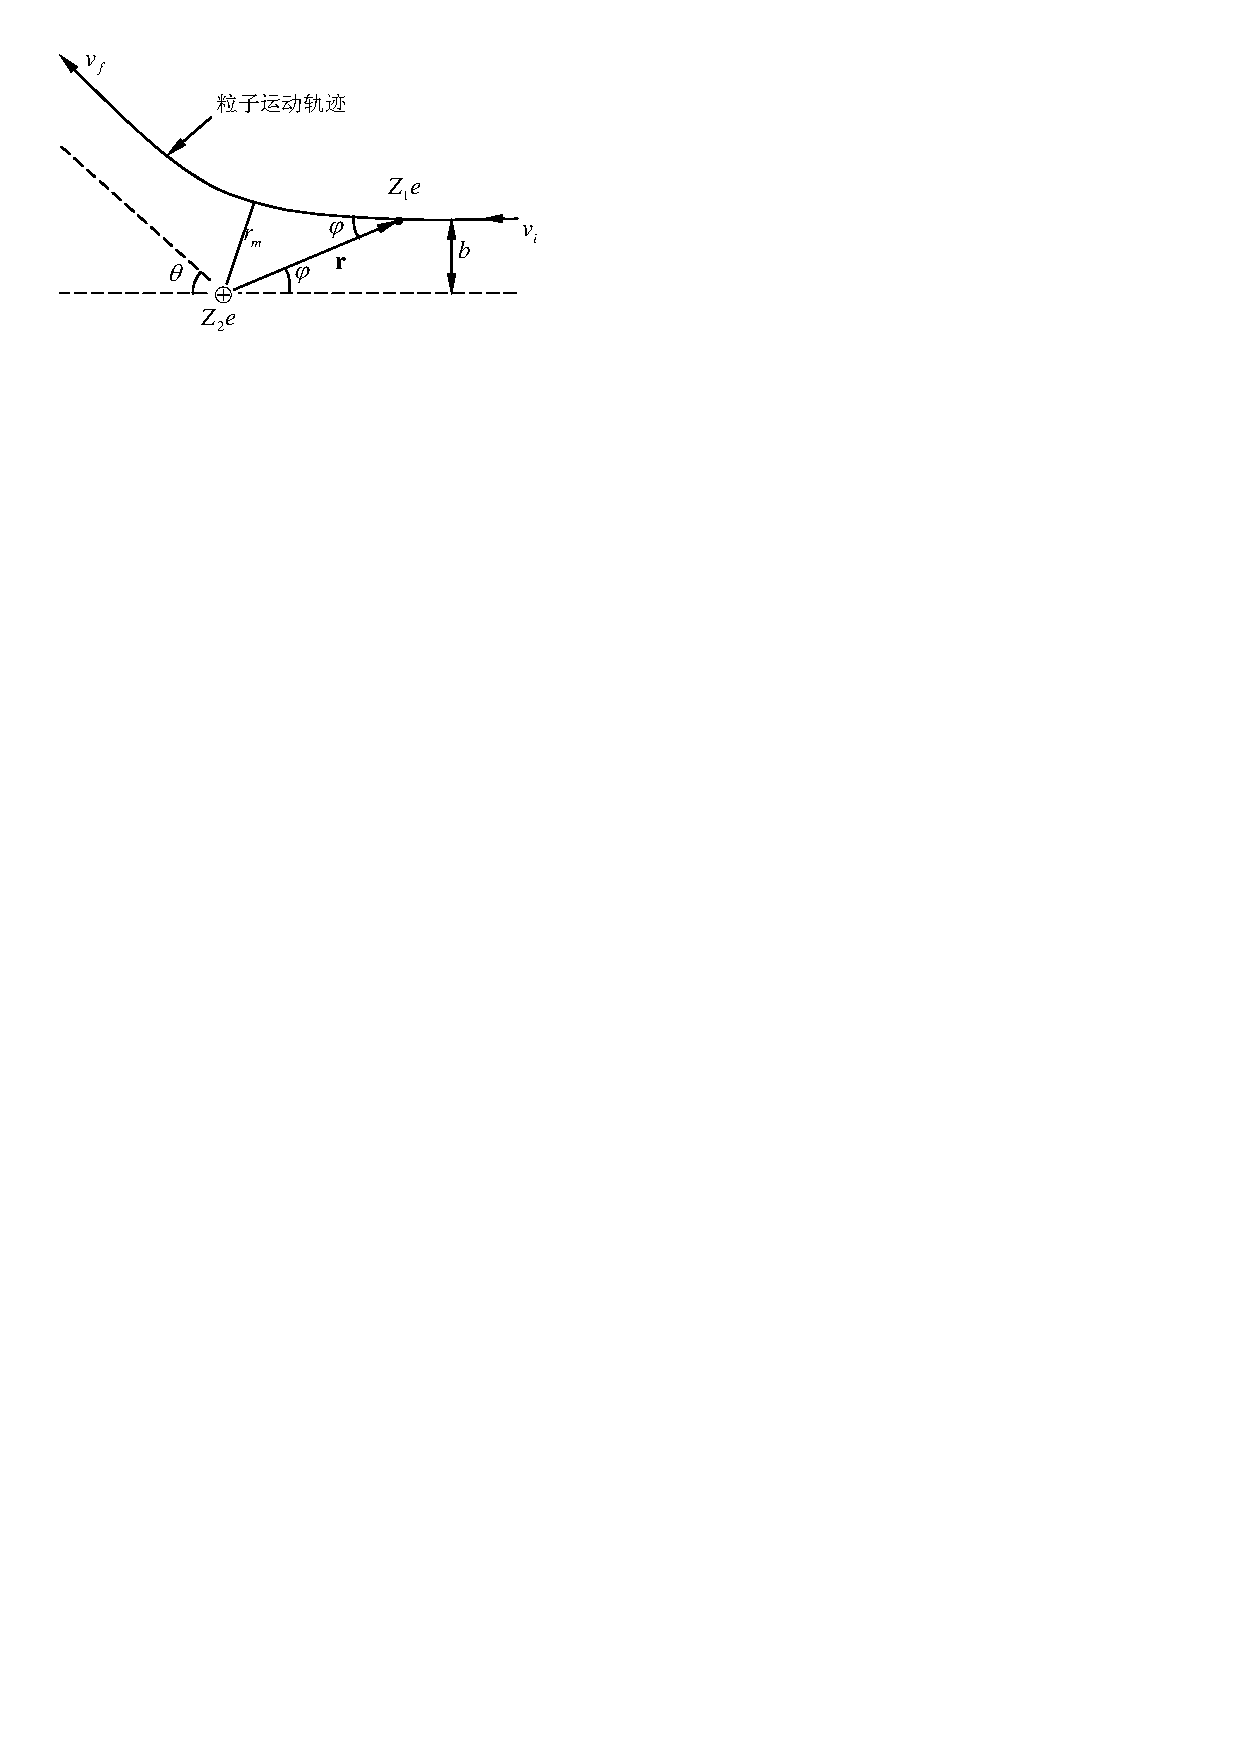
\includegraphics[width=0.5\textwidth]{fig01.pdf}
\caption{库仑散射}
\end{figure}
\end{itemize}

\subsection{卢瑟福公式及推导}
\begin{itemize}
\item \textbf{公式}: 微分截面$\sigma_c$为
\[
\sigma_c(\theta)=\Big(\frac{1}{4\pi\varepsilon_0}\frac{Z_1Z_2e^2}{4E}\Big)^2\frac{1}{\sin^2\frac{\theta}{2}}
\]
\item \textbf{推导}: 由库仑散射公式可知,瞄准距在$b$到$b+\textrm{d}b$之间的$\alpha$
粒子,经过散射必定向$\theta$到$\theta-\textrm{d}\theta$之间的角度射出. 设一薄箔的面积为$A$
,厚度为$t$(薄箔中的原子互相不遮蔽),环的面积为$2\pi
b|\textrm{d}b|$ ,则粒子打在这个环上的几率为
\[
\frac{2\pi
b|\textrm{d}b|}{A}=\frac{2\pi}{A}\Big(\frac{a}{2}\cot\frac{\theta}{2}\Big)
\Big|-\frac{a}{2}\csc^2\frac{\theta}{2}\cdot\frac{1}{2}\textrm{d}\theta\Big|
=\frac{a^22\pi
\sin\theta\textrm{d}\theta}{16A\sin^4\frac{\theta}{2}}
\]
由图\ref{fig02}可知,空心圆锥体的立体角与$\textrm{d}\theta$有: 
\[
\textrm{d}\Omega=\frac{2\pi r\sin\theta\cdot
r\text{d}\theta}{r^2}=2\pi \sin\theta\textrm{d}\theta
\]
由以上两式得
\[
\frac{2\pi
b|\textrm{d}b|}{A}=\frac{a^2\textrm{d}\Omega}{16A\sin^4\frac{\theta}{2}}
\]

一个薄箔有许多这样的圆环: 对应于一个原子核就有一个环;假如在单位体积内的原子核数为
$n$,则在体积$At$内共有$nAt$个环. 故被散射到$\theta$到
$\theta-\textrm{d}\theta$范围的几率为
\[
\textrm{d}p(\theta)=\frac{a^2\textrm{d}\Omega}{16A\sin^4\frac{\theta}{2}}nAt
\]
若有$N$个$\alpha$粒子打在薄箔上,则在$\textrm{d}\Omega$方向上测量到的$\alpha$
粒子数应为
\[
\textrm{d}N'=N\frac{a^2\textrm{d}\Omega}{16A\sin^4\frac{\theta}{2}}nAt
=ntN\Big(\frac{1}{4\pi\varepsilon_0}\frac{Z_1Z_2e^2}{4E}\Big)^2\frac{\textrm{d}\Omega}{\sin^4\frac{\theta}{2}}
\]
定义微分截面: 
\[
\sigma_c(\theta)=\Big(\frac{1}{4\pi\varepsilon_0}\frac{Z_1Z_2e^2}{4E}\Big)^2\frac{1}{\sin^2\frac{\theta}{2}}
\]

\begin{figure}[!htb]
\centering
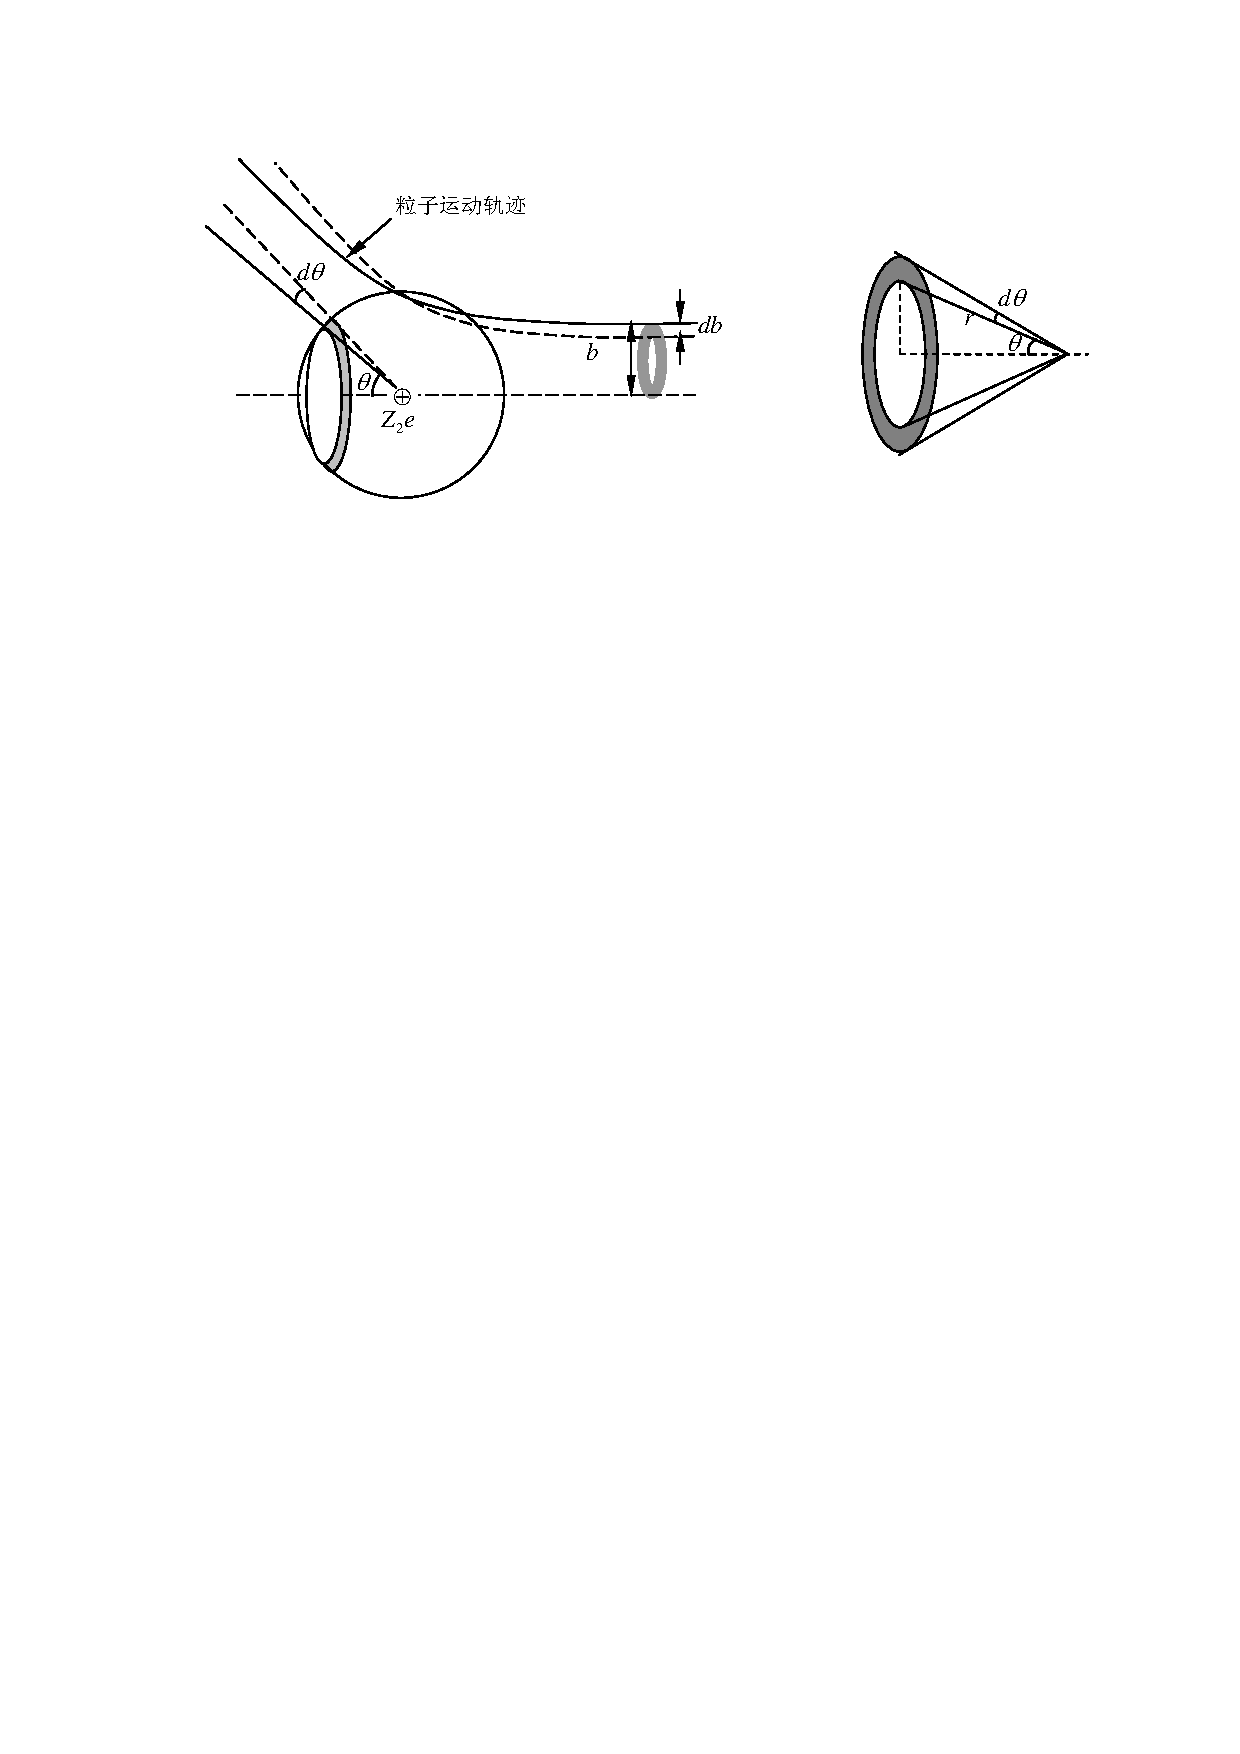
\includegraphics[width=0.7\textwidth]{fig02.pdf}
\caption{\label{fig02}卢瑟福公式}
\end{figure}
\item \textbf{意义}: $\sigma_c(\theta)$具有面积的量纲,它的物理意义是,$\alpha$粒子散射到$\theta$方向单位立体角内每个原子的有效散射截面. 
\end{itemize}

\subsection{行星模型的困难?}
\begin{multicols}{2} 
课本中有这样一段话(P25): ``谁都知道,任何带电粒子在作加速运动的过程中都要以发射电磁波方式放出能量. 这样, 电子就不能永远绕原子核转下去
. ''这句话对吗?

\begin{center}
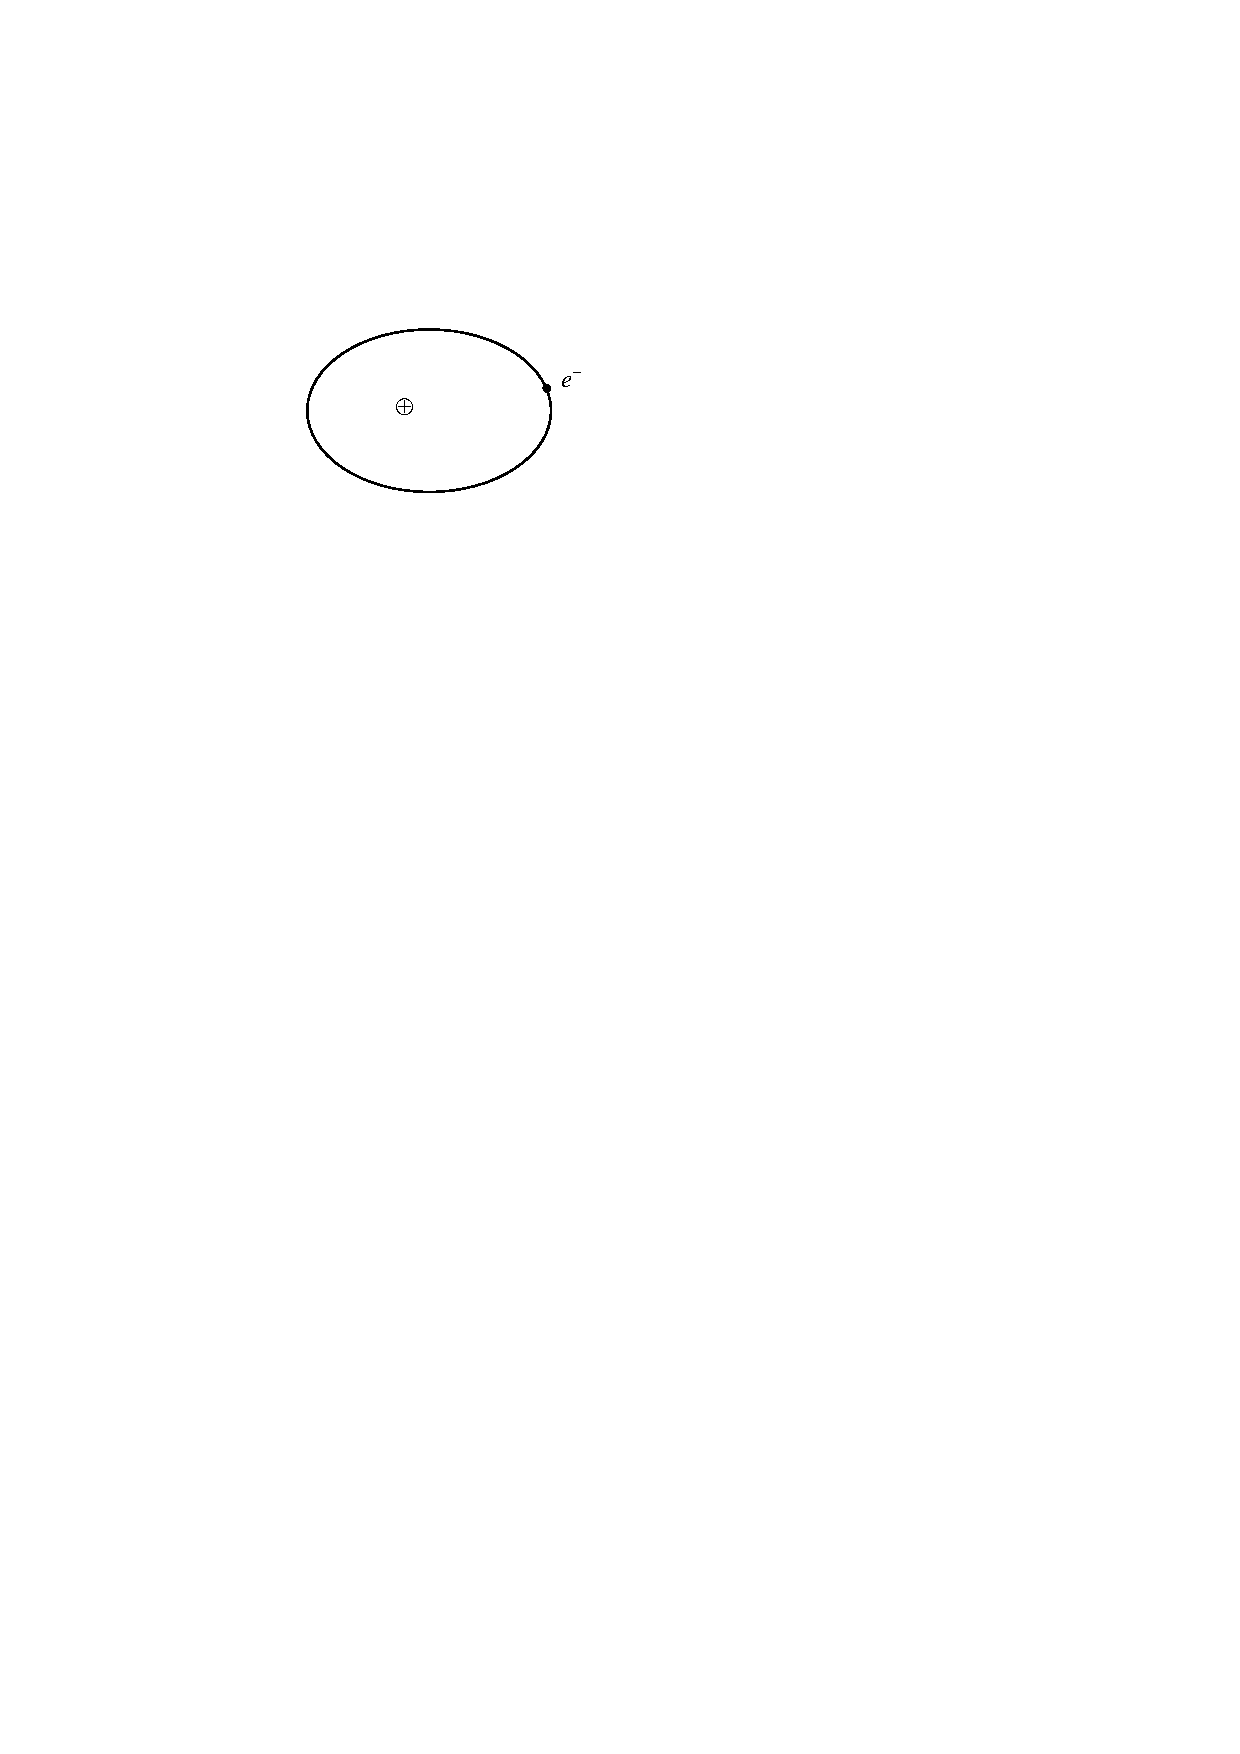
\includegraphics[width=0.175\textwidth]{fig15.pdf}
\end{center}
\end{multicols}

\vspace{-1em}
从经典力学出发,讨论行星模型电子到底能不能永远绕原子核转下去. 对原子系统,外力忽略不计,则有
\[
\textrm{没有能量交换}\Longrightarrow\frac{\textrm{d}E_{atom}}{\textrm{d}t}=0
\]
\[
\sum
\overrightarrow{r_{ic}}\times\overrightarrow{f_i^e}=\frac{\textrm{d}\sum\overrightarrow{r_{ic}}\times
m_i\dot{\overrightarrow{r_{ic}}} }{\textrm{d}t}=0
\quad \Longrightarrow\quad
\textrm{角动量}\sum\overrightarrow{r_{ic}}\times
m_{i}\dot{\overrightarrow{r_{ic}}}=\overrightarrow{C}\textrm{常矢量}
\]
结果与课本中的结论相反,这与我们所知道的: 地球绕了太阳几亿年也没落到太阳上一样. 

\newpage
\section{原子的量子态: 玻尔模型}
\subsection{光电效应}
光电效应中的能量关系: 
\[
\frac{1}{2}mv_m^2=hv-\phi
\]
其中$\frac{1}{2}mv_m^2$为逸出电子的最大动能, $\phi$为逸出功. \textbf{思考}: 当金属带有不同电量时, 上式能否成立, 为什么?

\subsection{玻尔(Bohr)模型}
氢原子中的一个电子绕原子核作圆周运动(经典轨道), 电子只能处于一些分立的轨道上, 它只能在这些轨道上绕核转动, 且不产生电磁辐射. 玻尔模型中的辐射条件:  $h\nu=E_{n'}-E_n$

\subsection{氢光谱}
根据氢原子辐射谱线的巴耳末公式, 里德伯提出了里德伯方程, 氢的所有谱线都可用这个方程表示
\[
\tilde{\nu}=\frac{1}{\lambda}=\frac{1}{B}\Big(\frac{1}{n^2}-\frac{1}{n'^2}\Big),\quad n=3,4,5\cdots,\quad n'=n+1,n+2,n+3\cdots
\]
图\ref{fig03}是氢原子轨道和光谱线示意图.
\begin{figure}[!htb]
\centering
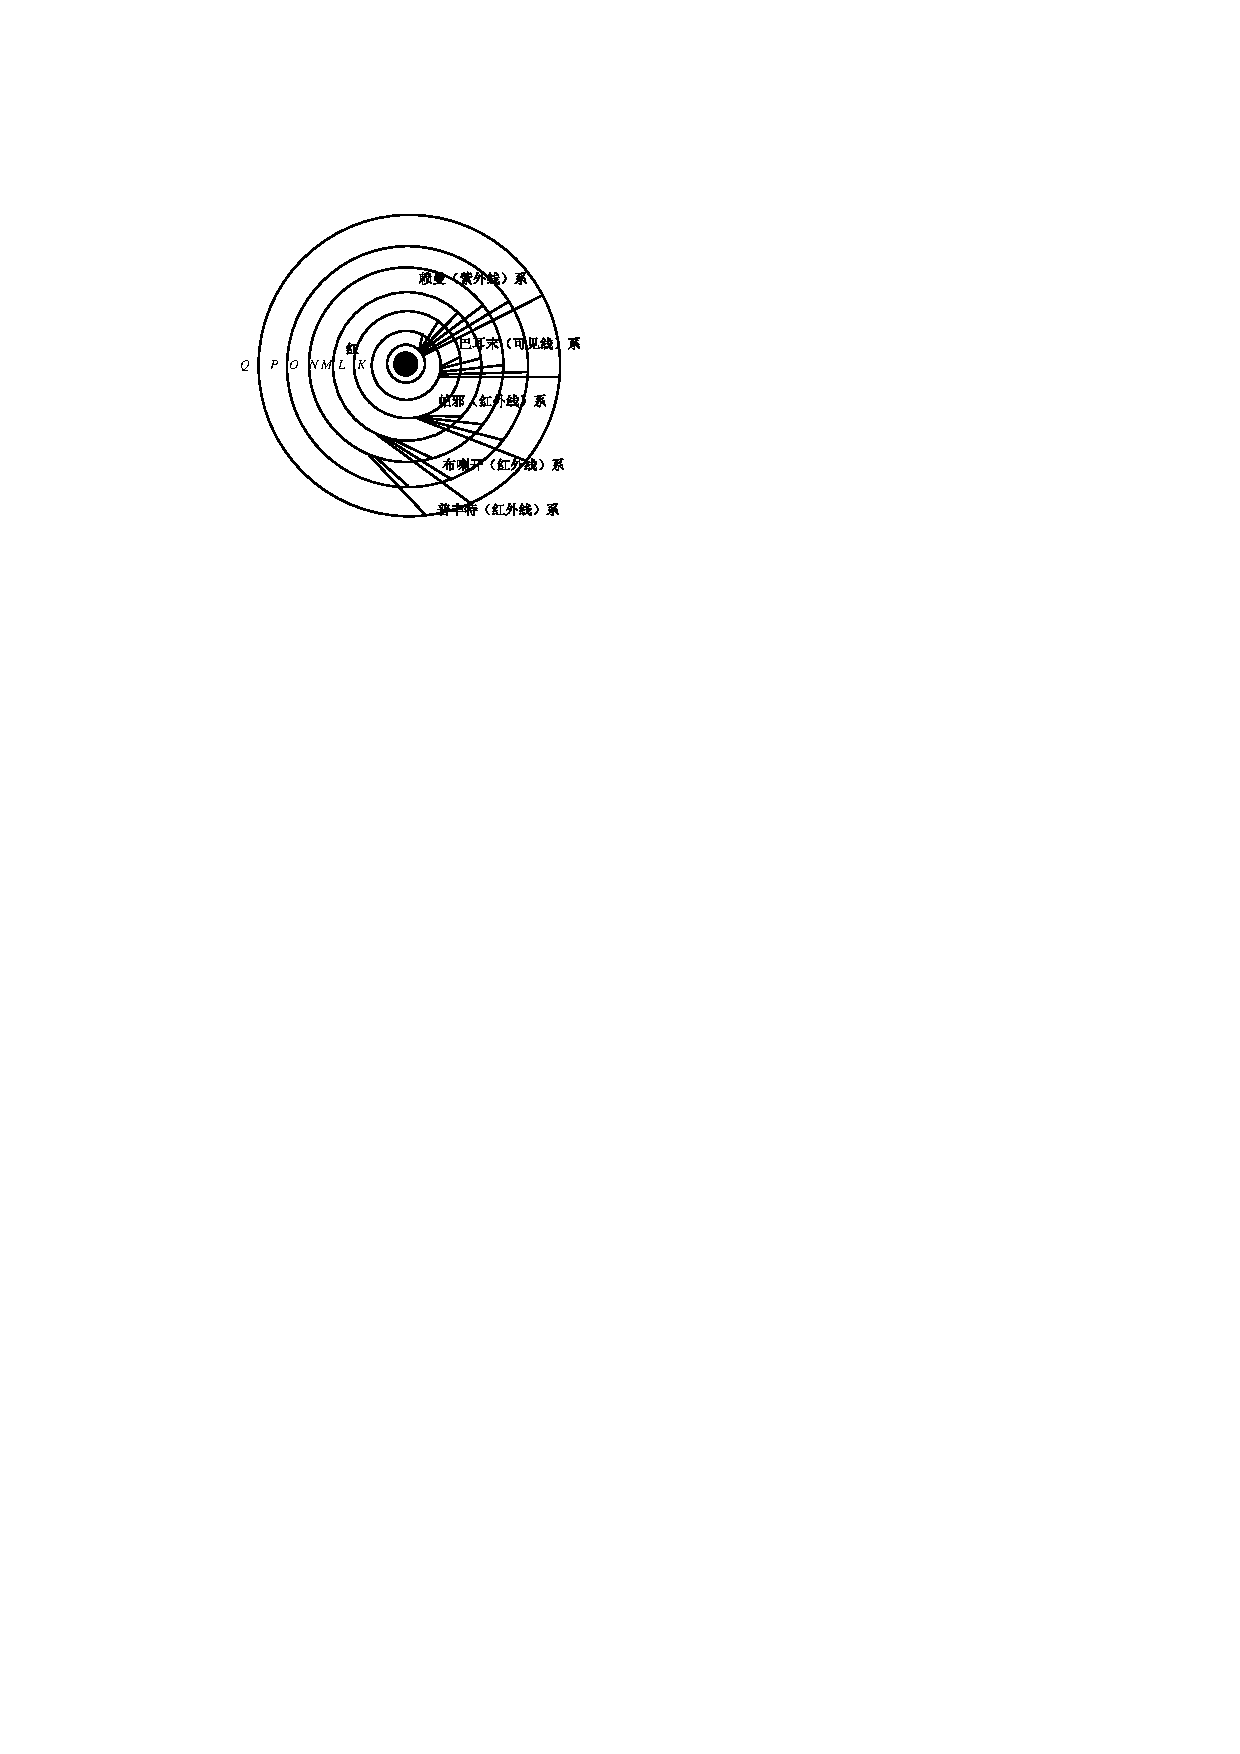
\includegraphics[width=0.3\textwidth]{fig03.pdf}
\caption{\label{fig03}原子轨道和光谱线示意图}
\end{figure}


\subsection{固, 液, 气光谱的成因特点}
\begin{itemize}
\item 固体: 固体光谱是晶格放的光形成的, 但晶格的联系太紧密, 故很少显示出原子状态跃迁发光. 固体光谱为连续谱. 
\item 液体: 液体光谱更多的是分子之间的相互运动, 很少显示出跃迁发光(干扰因素太多). 液体光谱为带状谱. 
\item 气体: 电子跃迁发光. 气体光谱为线状谱. 
\end{itemize}
\noindent[\textbf{思考}]: 要了解原子内部的信息, 为何选用冷光源?

\subsection{夫兰克(Frank)-赫兹(Hertz)实验}

\begin{multicols}{2} 

如右图所示, 电子从热阴极K发出, 经K与G间电场加速. 在G与A之间加反电压, 当电子进入GA空间时, 若有较大能量, 则可以克服反电场到达极A. 若电子在KG区域把能量给了原子, 那么, 电子剩下的能量就不足以克服反电压而抵达A. \textbf{实验表明}: 汞原子对外来能量, 不是``来者皆收'', 而是以4.9eV为单位的吸收能量(气体状态下原子吸收电子的能量是不连续的).
%\begin{figure}[!htb]
%\centering
\begin{center}
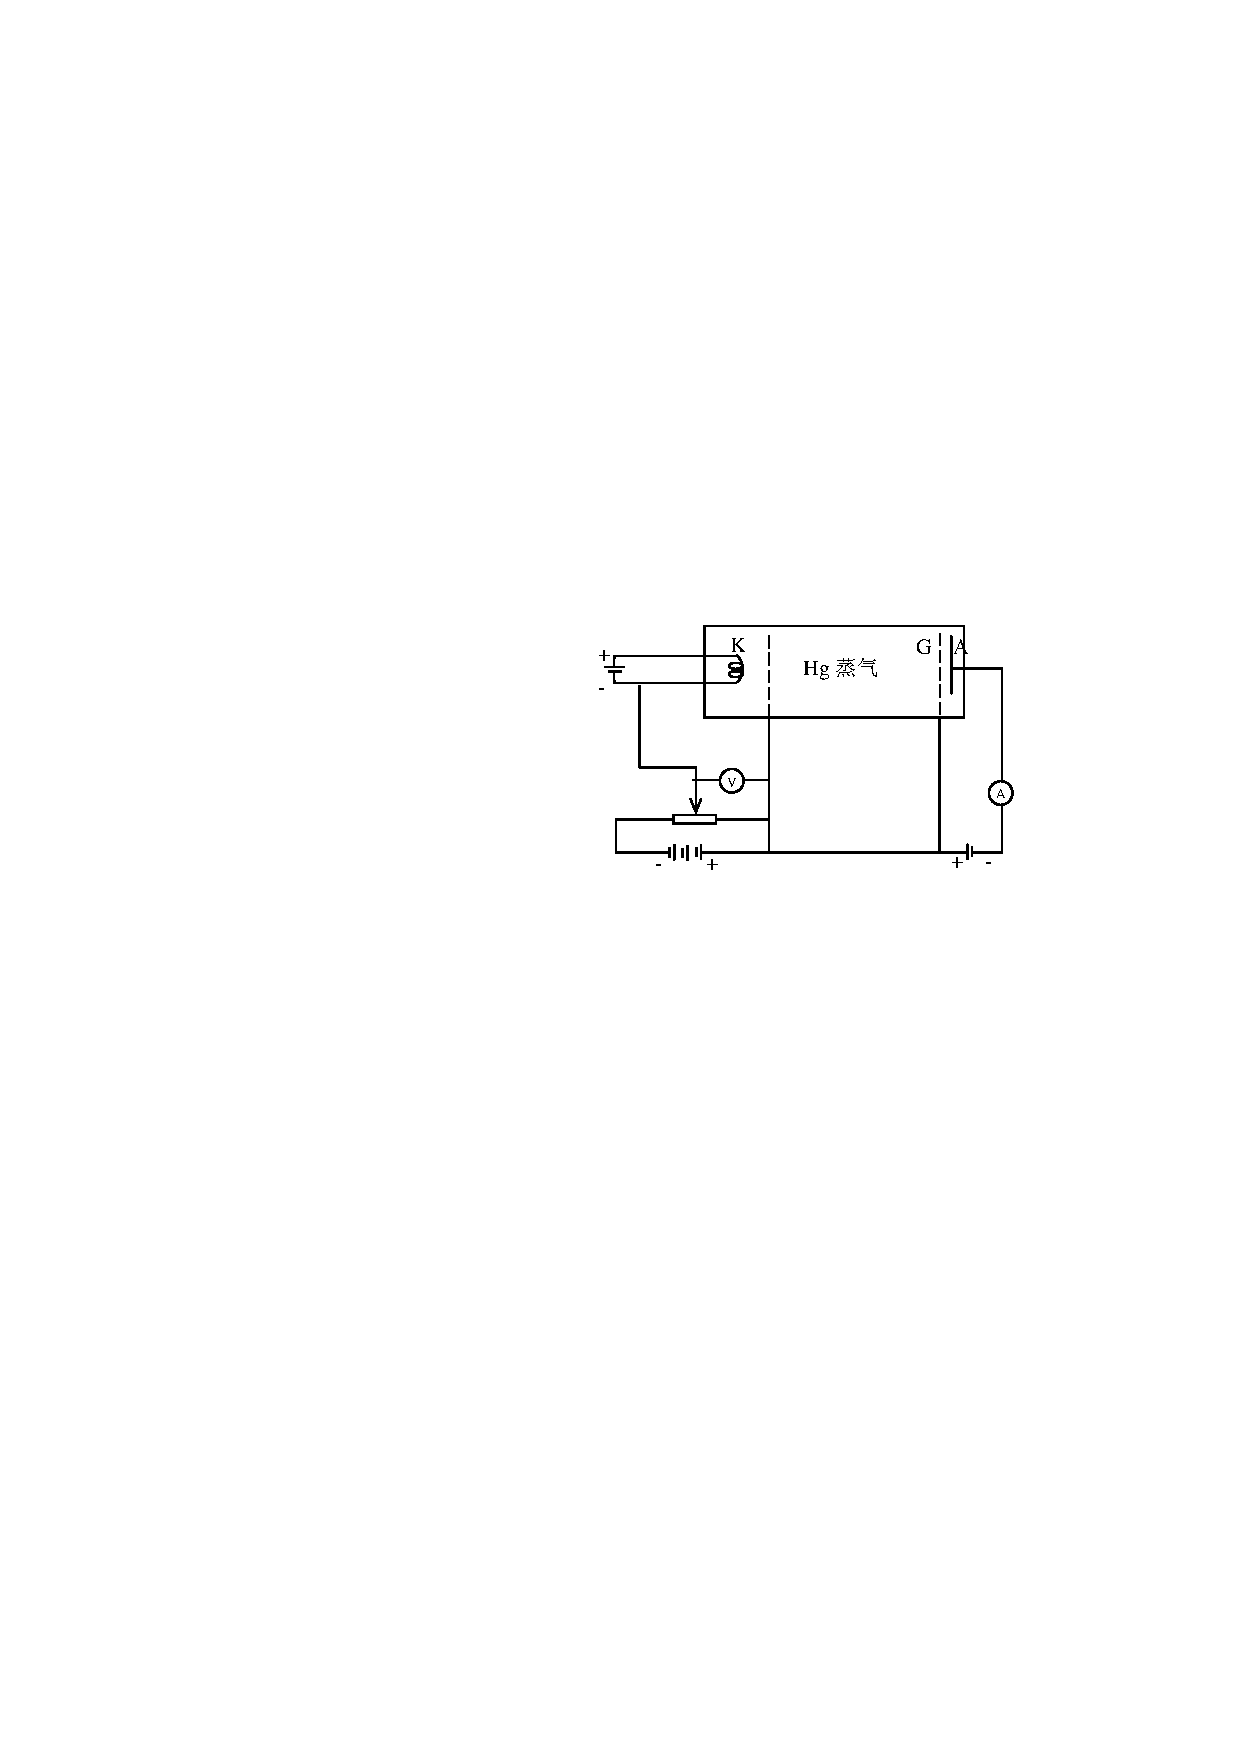
\includegraphics[width=0.3\textwidth]{fig04.pdf}
\end{center}
%\caption{\label{fig04}夫兰克-赫兹实验装置}
%\end{figure}
\end{multicols}


\newpage
\section{量子力学导论}
\subsection{德布罗(de Broglie)意波}
\begin{itemize}
\item \textbf{推导}: 由假设$E=h\nu$得
\[
E=h\nu=h\frac{1}{\tau^*}=h\frac{v}{v\tau^*}=h\frac{v}{\lambda} \ \
\footnote{偷换概念: $v\tau^*=\lambda$ ,其中$v$是粒子运动速度}
\]
又由爱因斯坦质能方程(亦属假设, 未证实): $E=mc^2$将光速$c$偷换为$v$得
\[
E=mv^2
\]
由以上两式联立可得
\[
\lambda=\frac{h}{mv}
\]
\item \textbf{结论}: 可见推导是有问题, 推导的前提依据都是假说, 并且推导本身就有问题. 
\end{itemize}
\subsection{波与粒子的区别}
粒子携带质量, 符合动力学公式;波不携带质量(目前没有证据表明波携带质量),符合波的传播公式.请\textbf{思考}: 
\begin{itemize}
\item 定量描述波与粒子的区别?
\item 波干涉中的确定因素与电子衍射实验中的不确定因素, 电子衍射实验能否证明电子具有波动性?
\end{itemize}

\subsection{戴维孙(Davisson)-革末(Germer)实验}
戴维孙-革末实验用盖革记数器控测各个方向, 发现了有强弱分布. 戴维孙-革末实验能否说电子具有波动性. 
\begin{figure}[!htb]
\centering
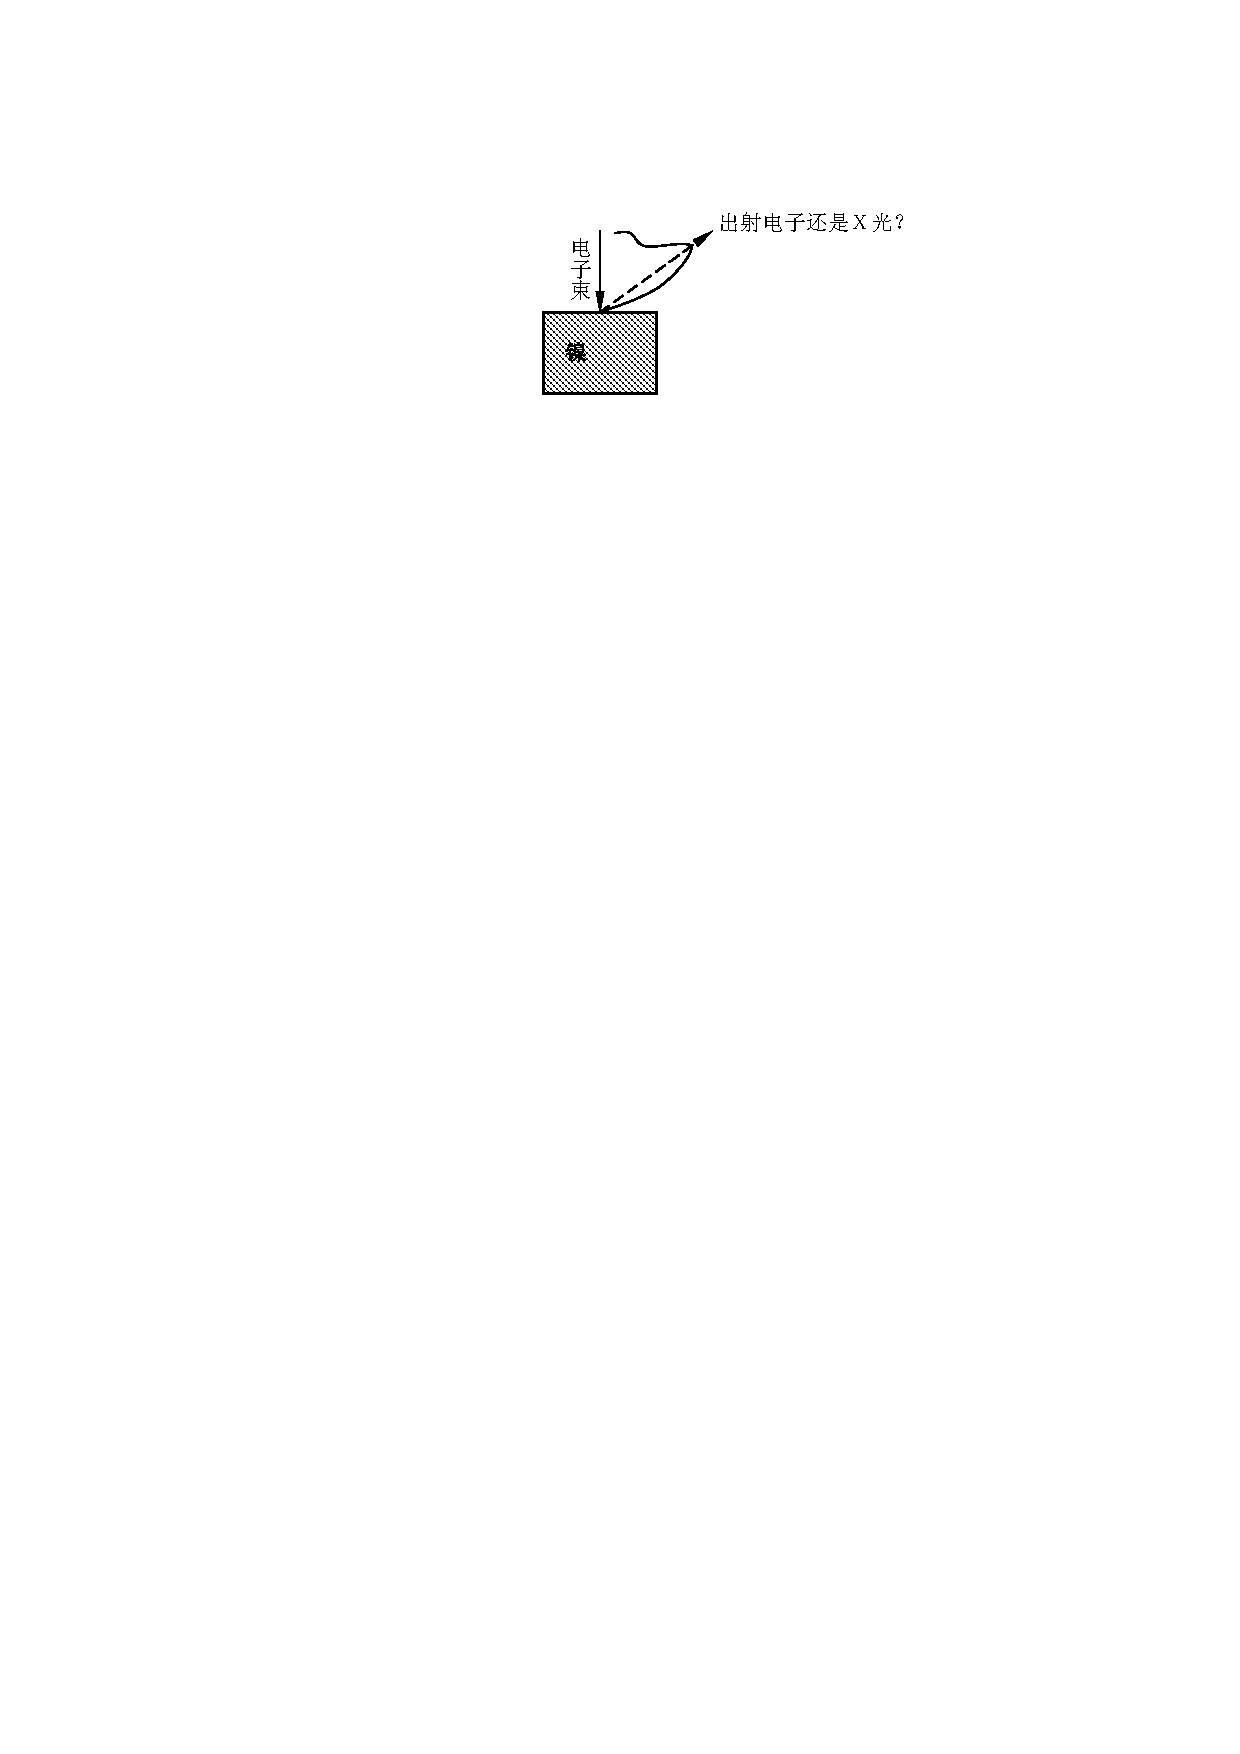
\includegraphics[width=0.4\textwidth]{fig16.pdf}
\caption{戴维孙-革末实验}
\end{figure}
事实上存在很大问题: 不能排除高能电子轰击材料而向各个方向上产生的x射线; 另外对于高能电子的轰击, 轰击后的速度几乎不可能与轰击前相同. 

\newpage
\section{原子的精细结构: 电子的自旋}
\subsection{史特恩(Stern)-盖拉赫(Gerlach)实验}
\begin{figure}[!htb]
\centering
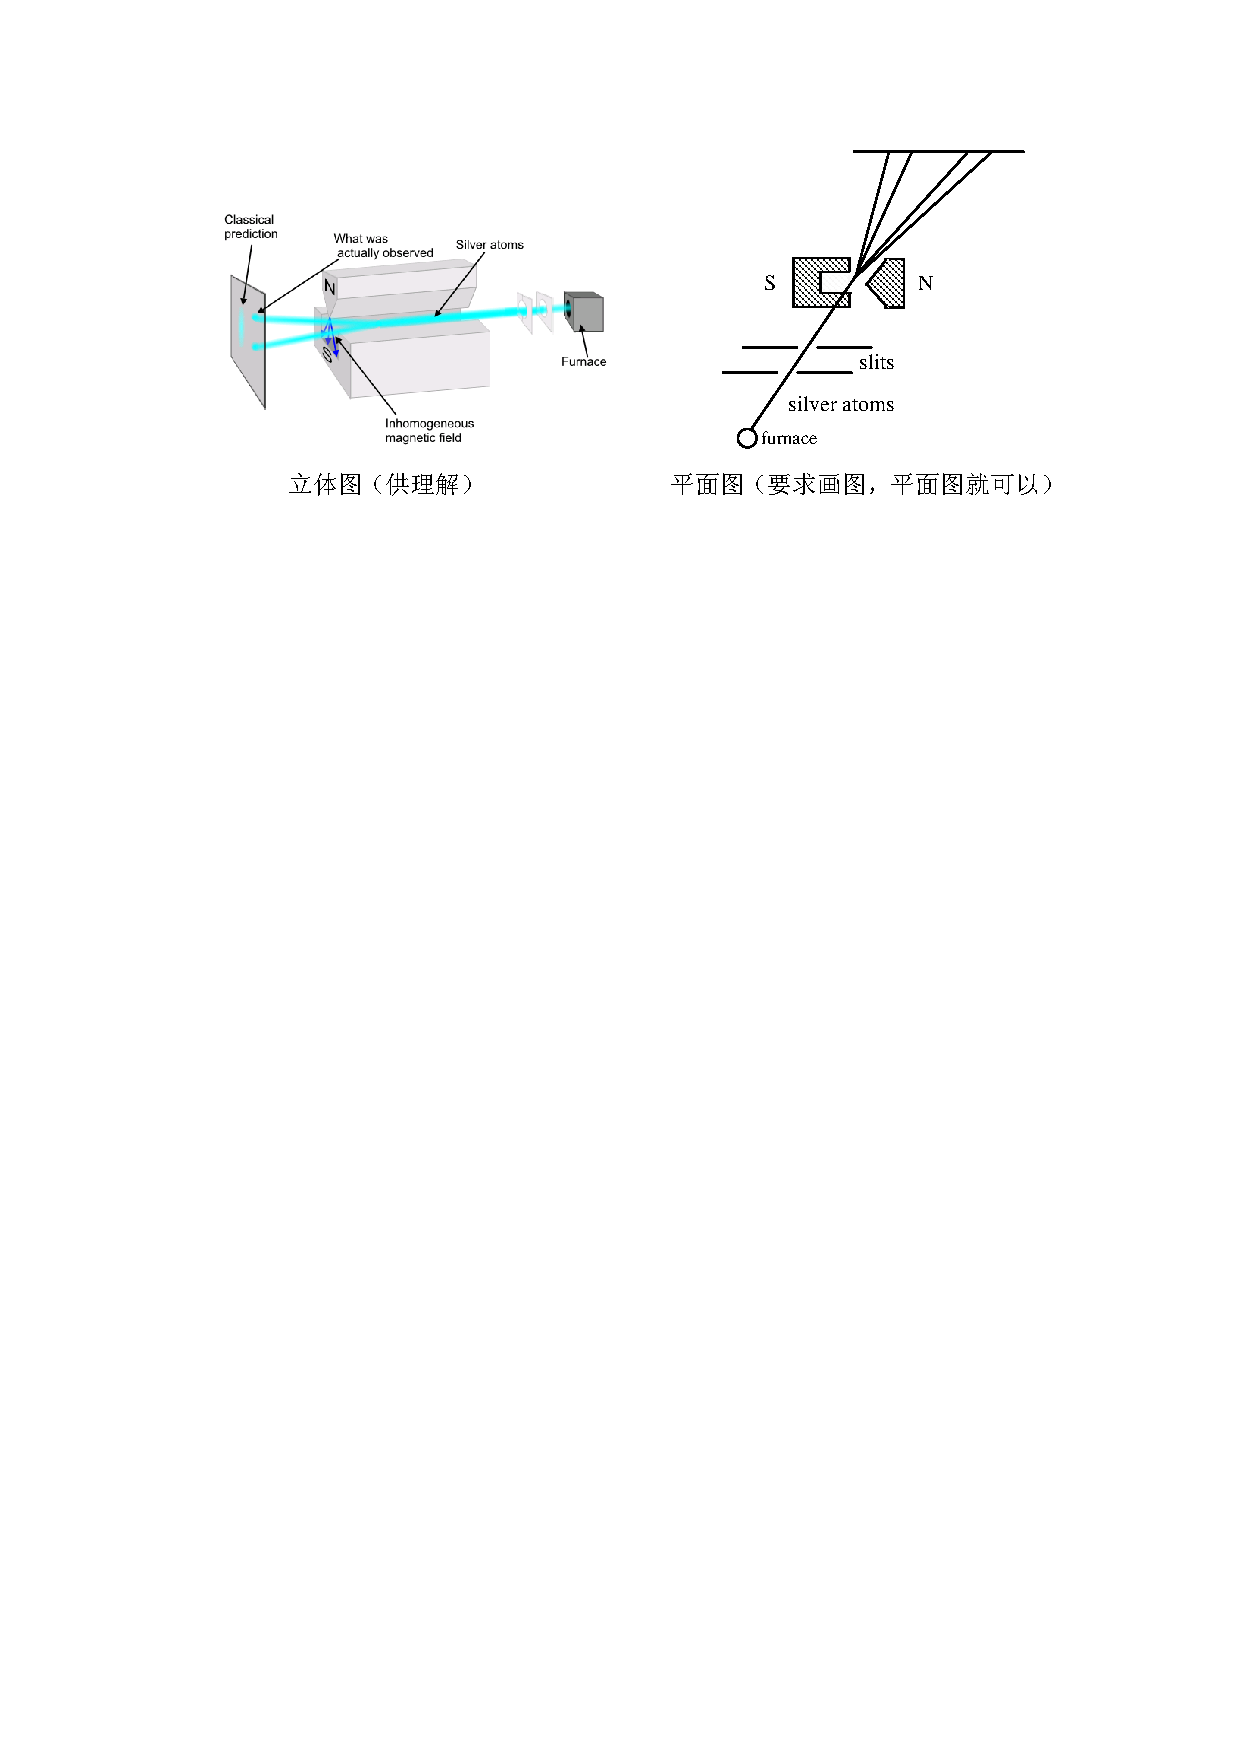
\includegraphics[width=0.8\textwidth]{fig05.pdf}
\caption{\label{fig05}特恩-盖拉赫实验}
\end{figure}
原子射线束通过一个不均匀的磁场区域, 射线束在磁场作用下发生偏折, 最后落在屏上. 如果原子磁矩的方向是可以任意取向的, 则屏上形成一片黑斑. 而实验发现屏上形成了几条清晰的黑斑, 表明银原子的\textbf{磁矩}($\mu$)只能取几个特定的方向, 从而验证了原子角动量的投影是量子化的.  在磁场中, 原子受力$f\varpropto\frac{\textrm{d}B}{\textrm{d}z}\mu$. \textbf{结果}如图\ref{fig06}.
\begin{figure}[!htb]
\centering
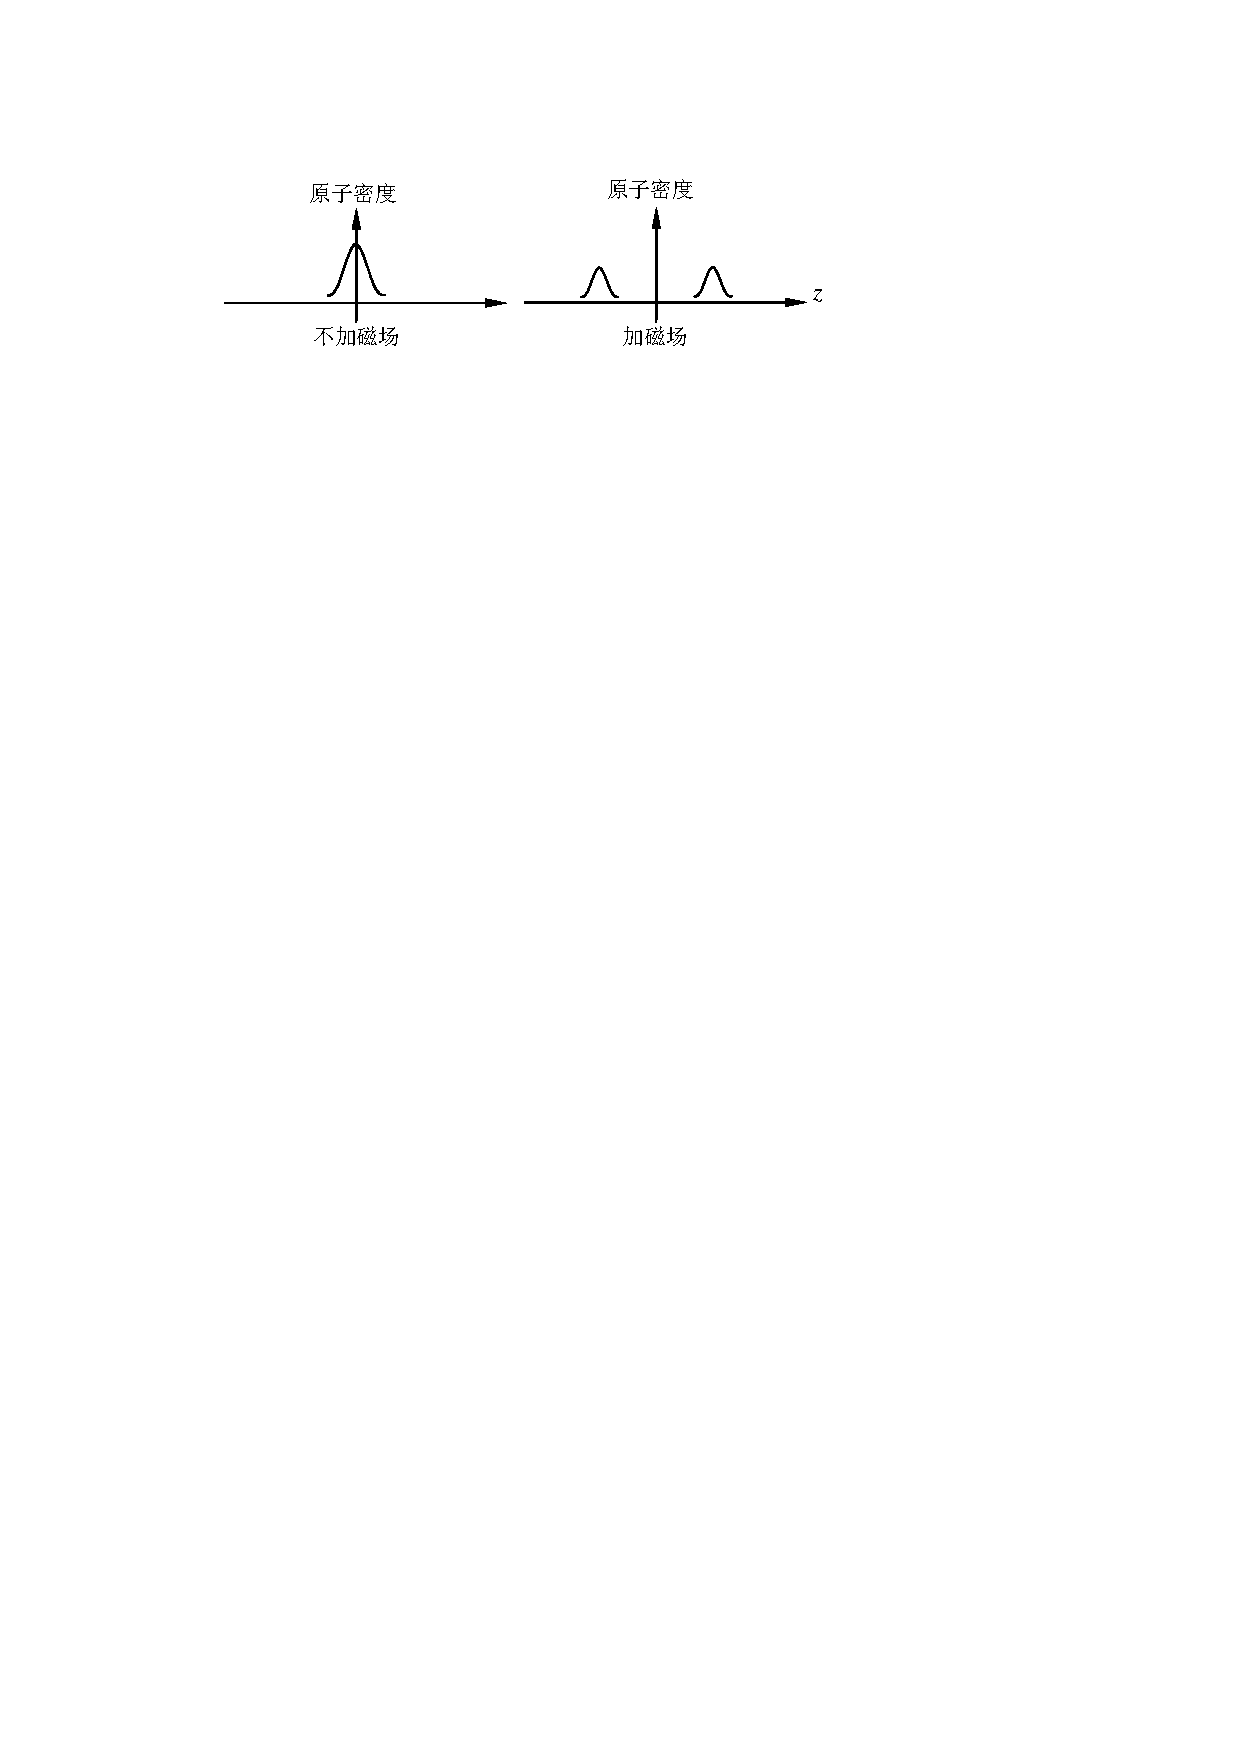
\includegraphics[width=0.6\textwidth]{fig06.pdf}
\caption{\label{fig06}史特恩-盖拉赫实验结果}
\end{figure}


\subsection{塞曼(Zeeman)效应}
塞曼效应是原子的光谱线在外磁场中出现分裂的现象. 
\begin{figure}[!htb]
\begin{minipage}[b]{0.48\textwidth}
\centering
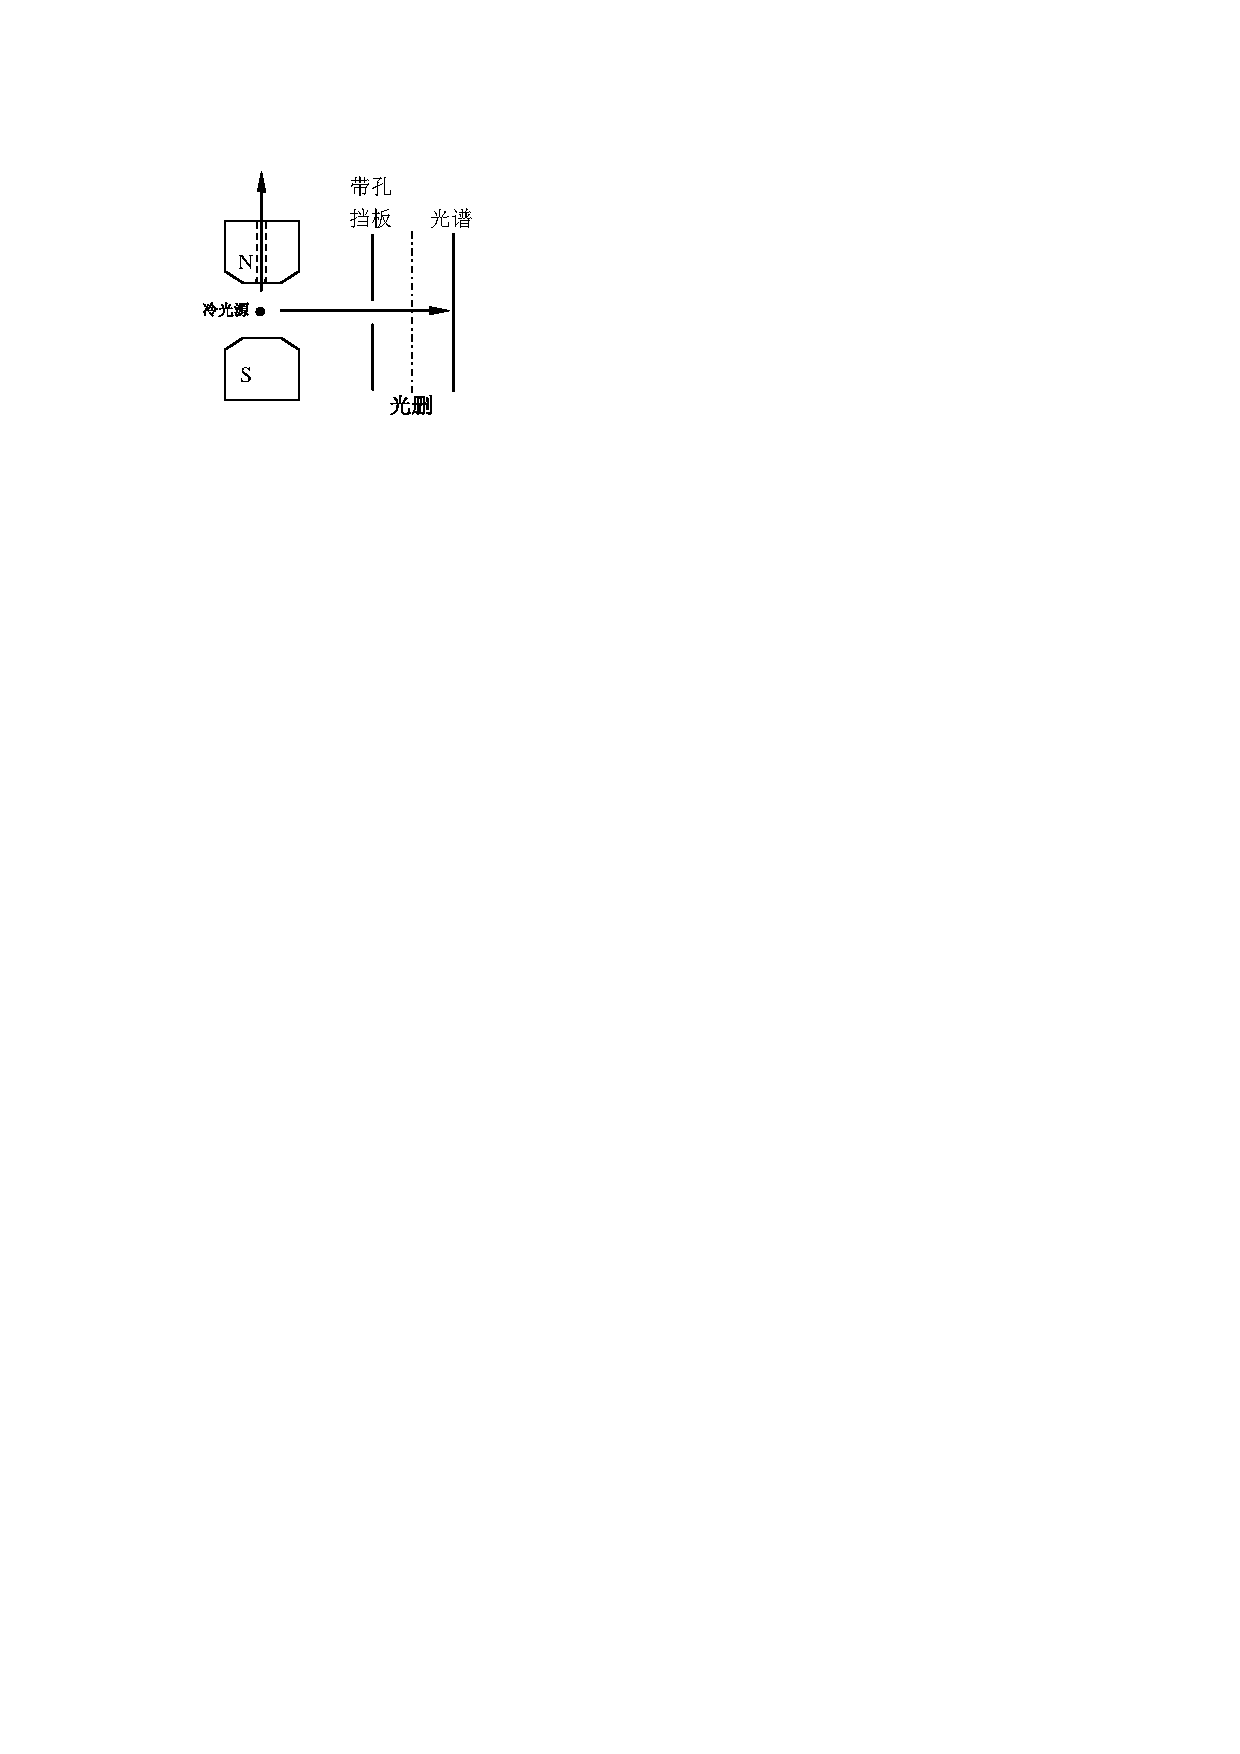
\includegraphics[width=0.7\textwidth]{fig07.pdf}
\caption{\label{fig08}塞曼效应实验装置}
\end{minipage}%
\begin{minipage}[b]{0.48\textwidth}
\centering
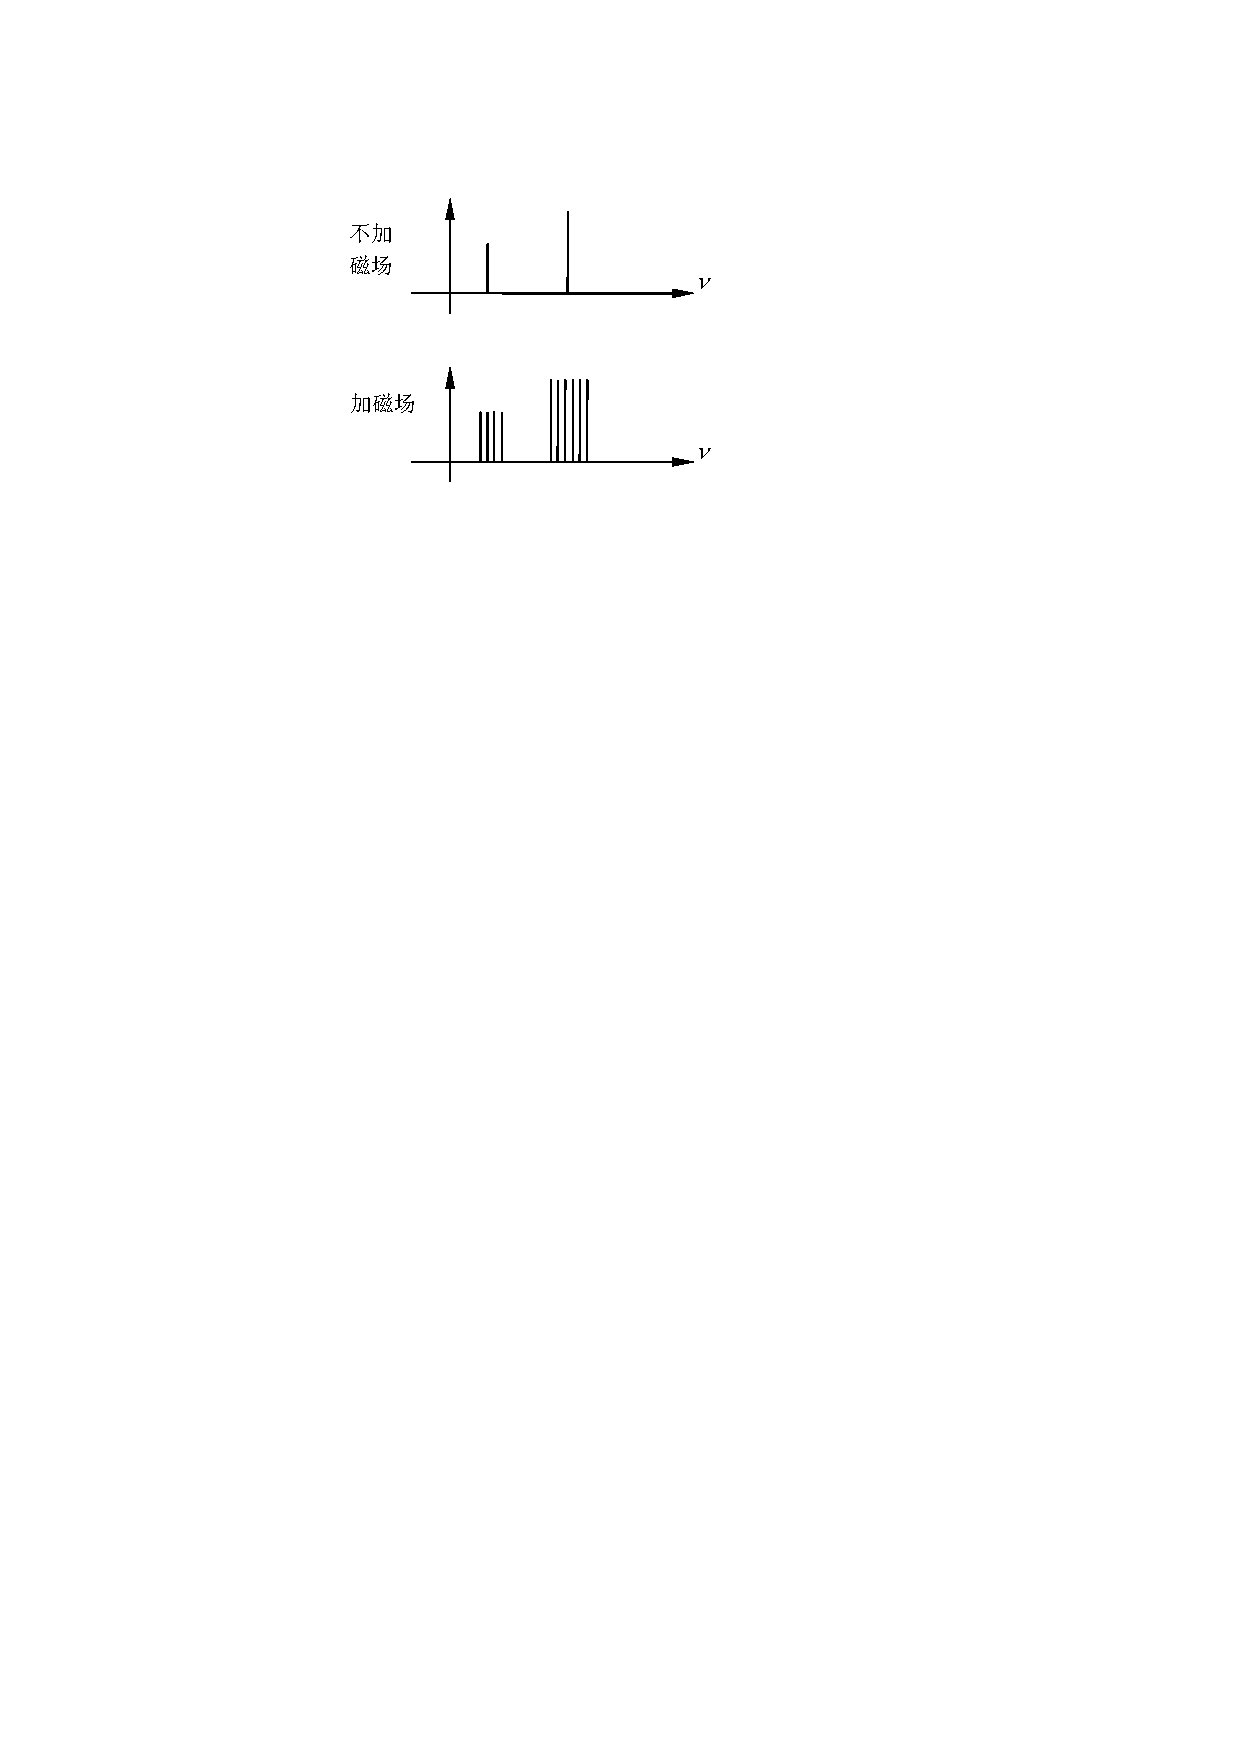
\includegraphics[width=0.7\textwidth]{fig14.pdf}
\caption{\label{fig09}塞曼效应的结果}
\end{minipage}
\end{figure}
\textbf{注意}: 塞曼效应的光谱为偏振光谱, 谱线对称分裂. 

\subsection{斯塔克(Stark)效应}
斯坦克效应是原子发出的谱线在电场作用下产生分裂的一种现象. 
\begin{figure}[!htb]
\begin{minipage}[b]{0.48\textwidth}
\centering
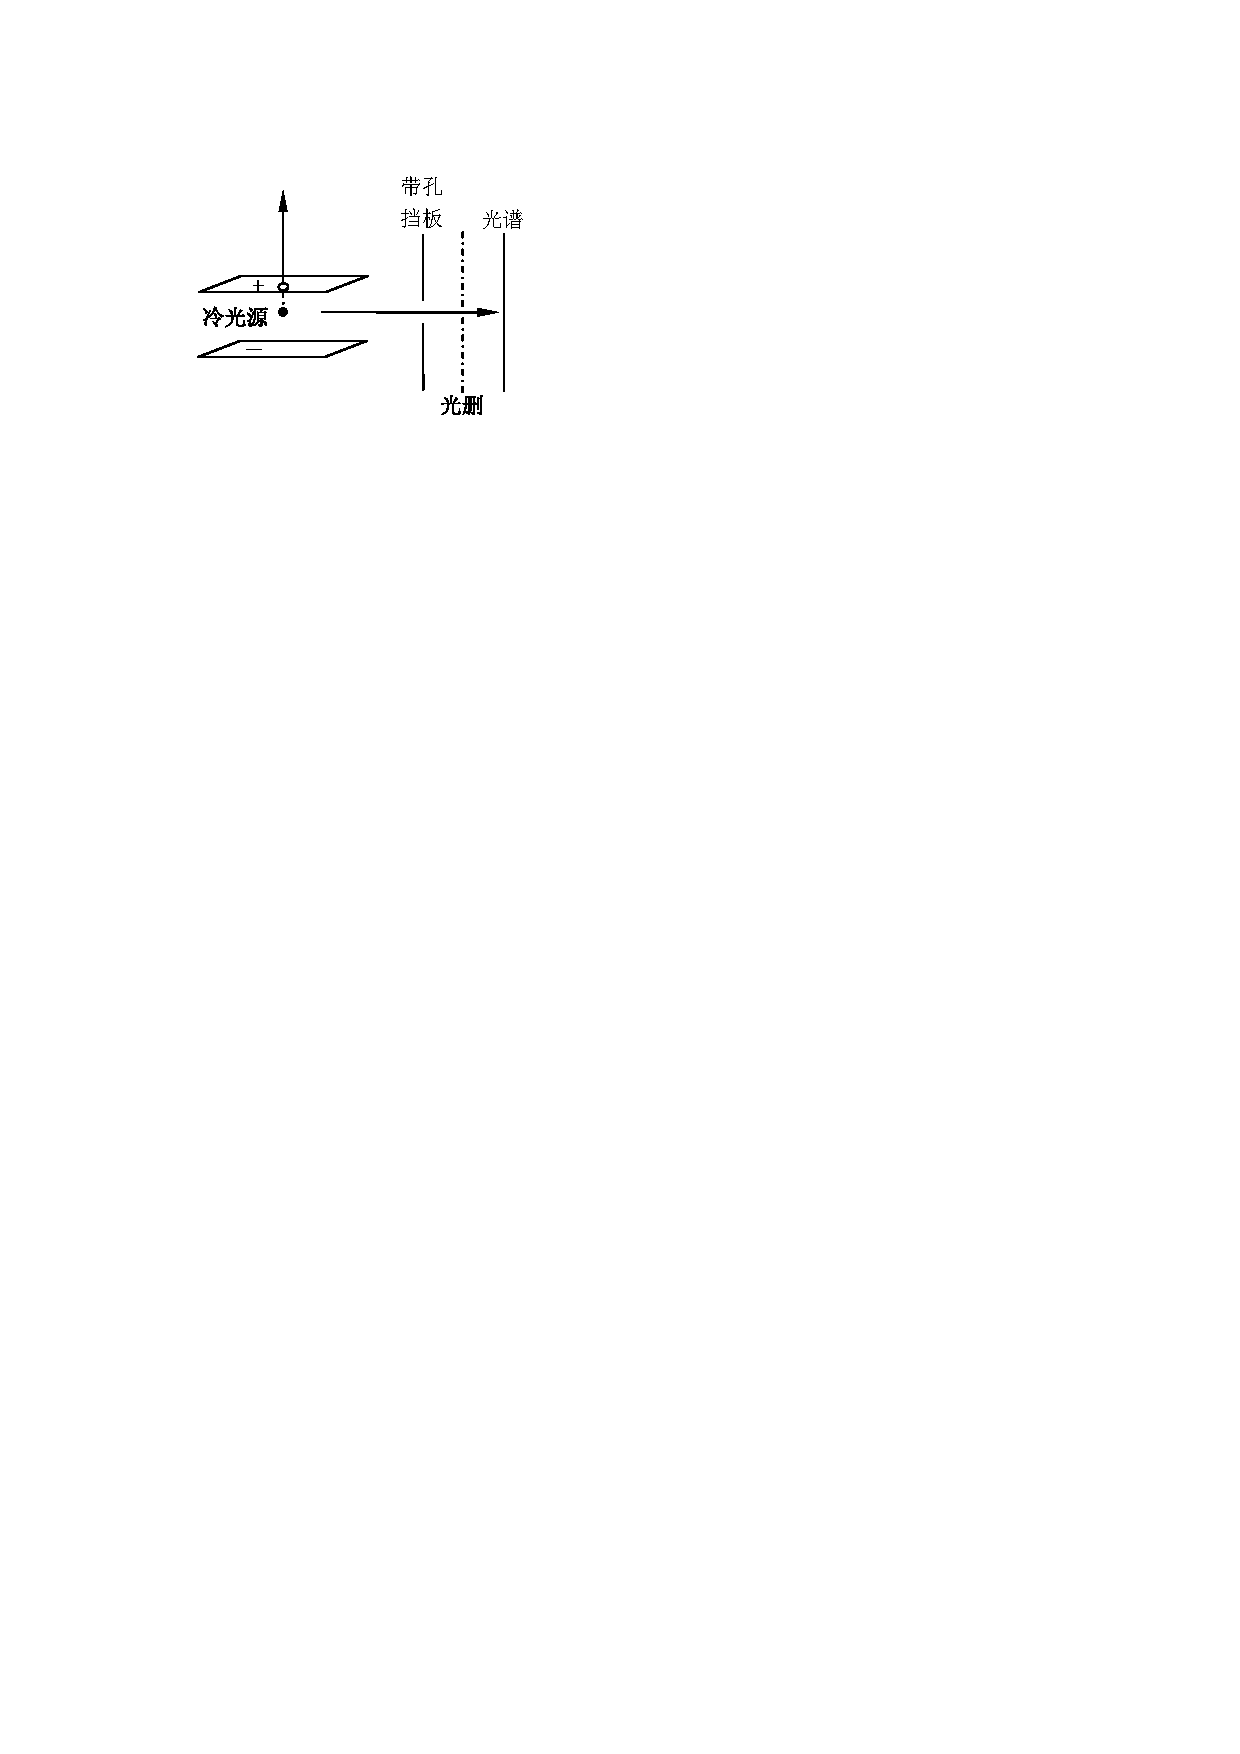
\includegraphics[width=0.7\textwidth]{fig08.pdf}
\caption{\label{fig08}斯坦克效应实验装置}
\end{minipage}%
\begin{minipage}[b]{0.48\textwidth}
\centering
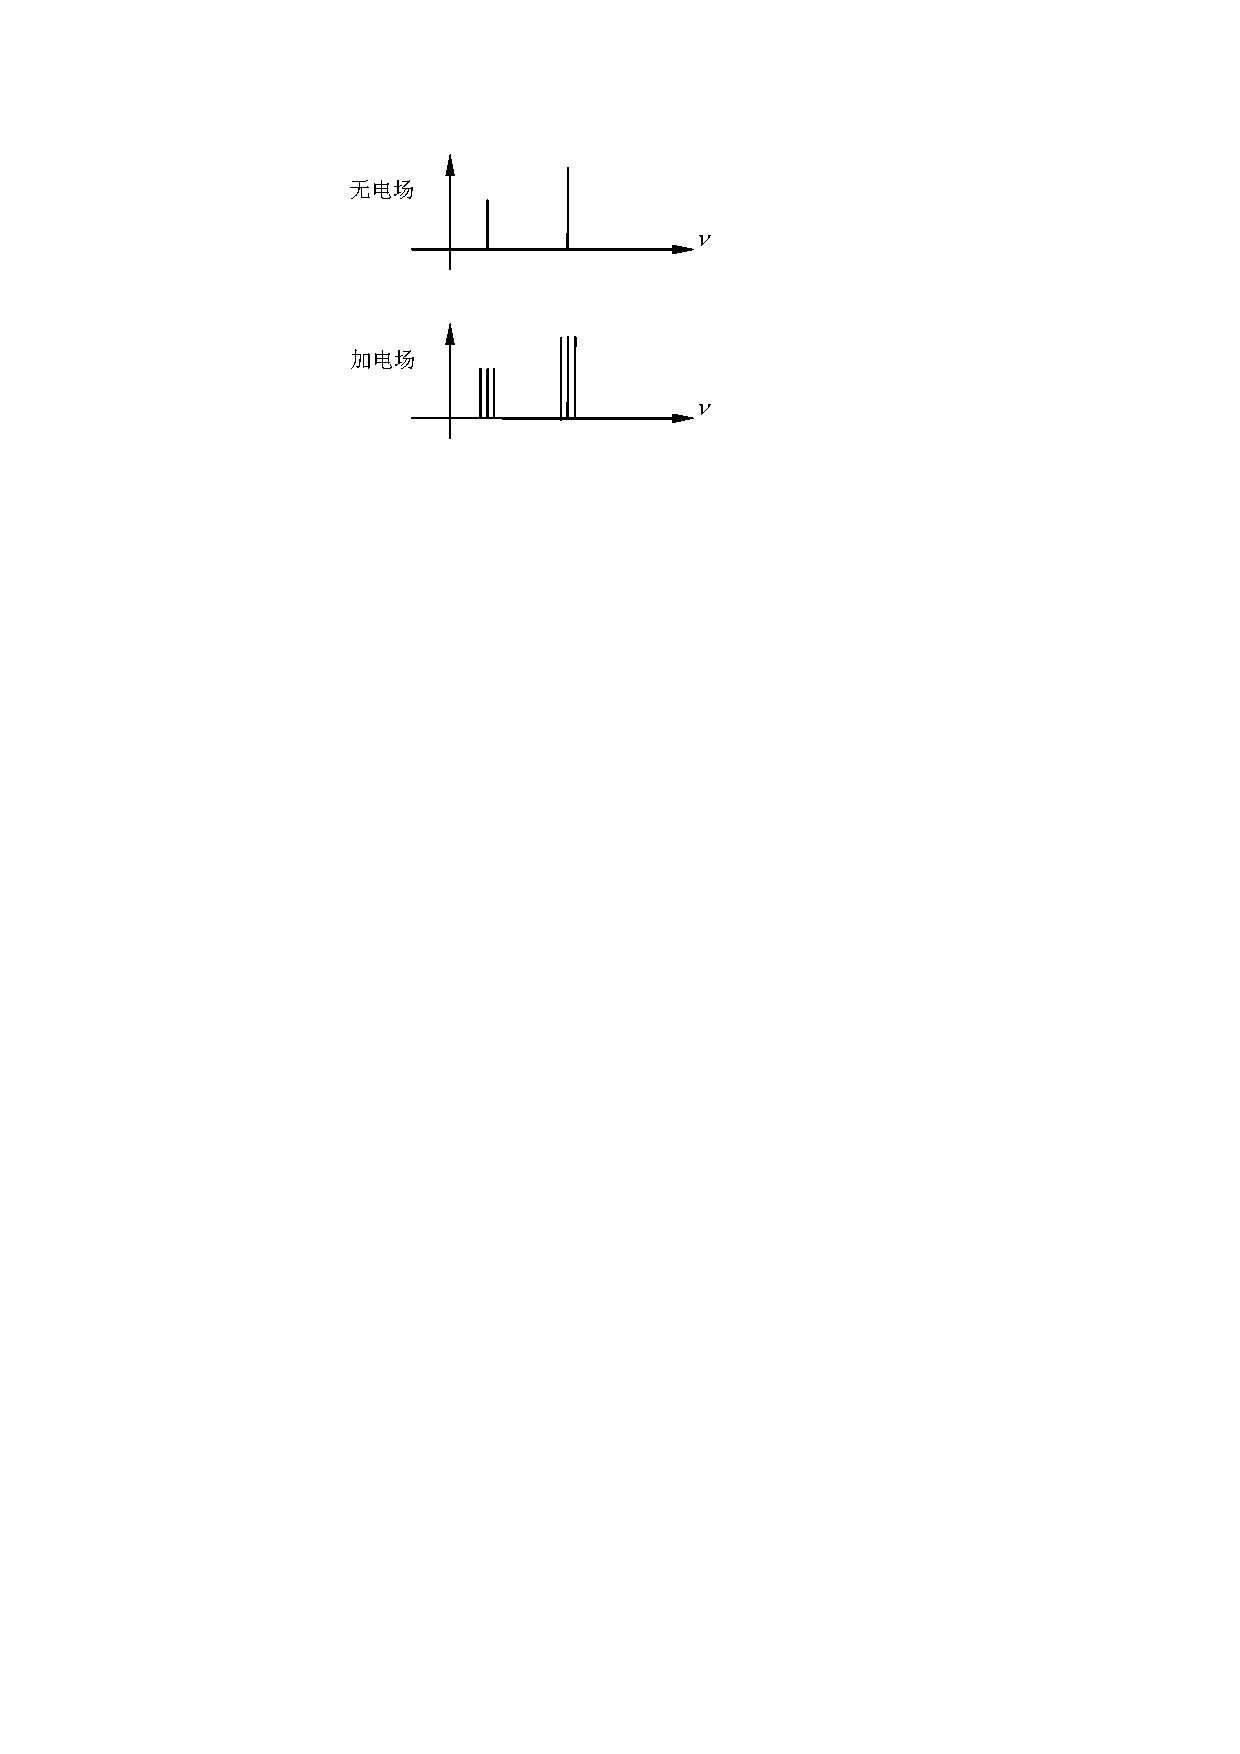
\includegraphics[width=0.7\textwidth]{fig09.pdf}
\caption{\label{fig09}斯坦克效应的结果}
\end{minipage}
\end{figure}
\textbf{结果}: 加电场后, 谱线由一条分裂成三条(如图\ref{fig09}), 并且对于氢原子有$\Delta\mu\propto E$(一级斯坦克效应)

\newpage
\section{多电子原子: 泡利原理}
\subsection{泡利(Pauli)不相容原理}
原子中每个状态只能容纳一个电子. 

\textbf{费米子(如电子)满足泡利不相容原理, 而玻色子(如光子)与泡利不相容原理无关. }

\section{X射线}
\subsection{莫塞雷(Moseley)实验}
用电子轰击不同的材料, 得到不同的X谱线. 
\begin{figure}[!htb]
\centering
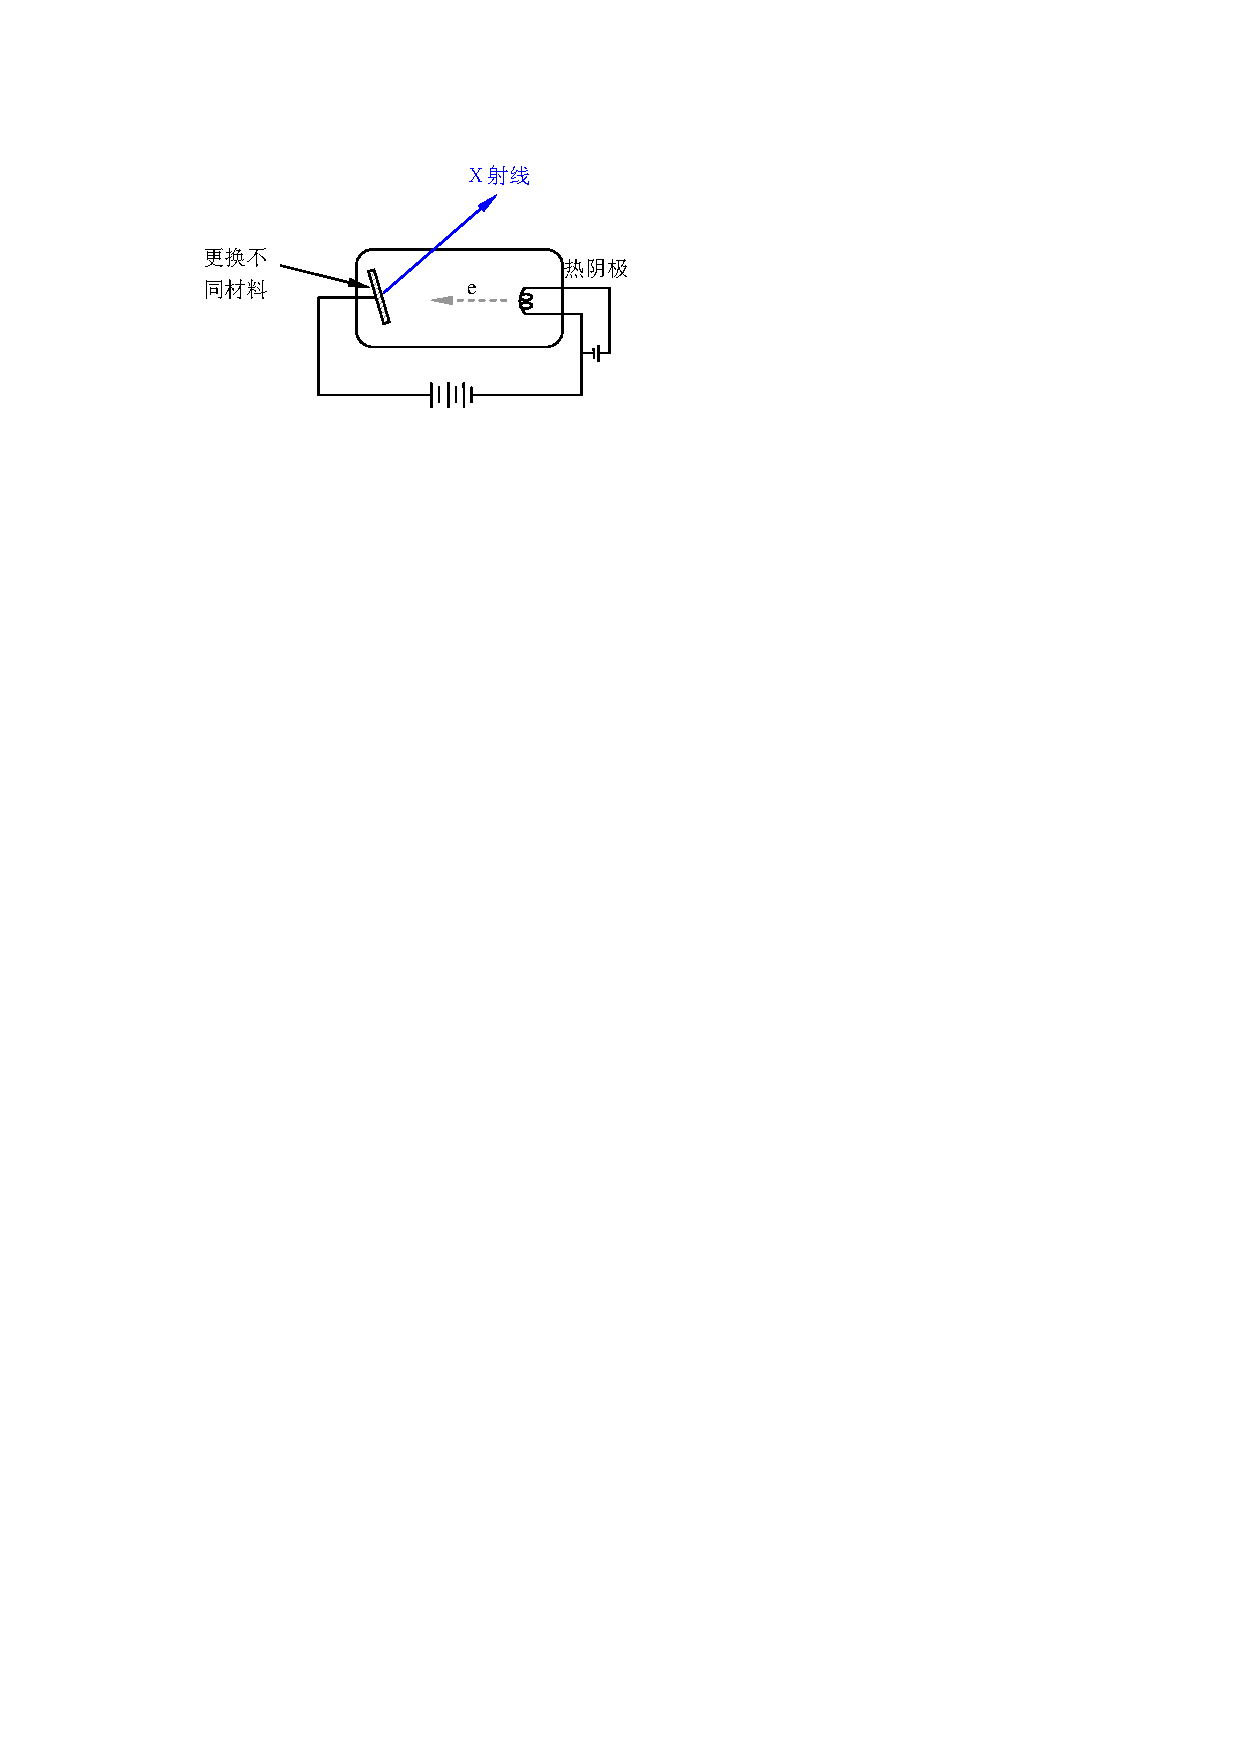
\includegraphics[width=0.5\textwidth]{fig10.pdf}
\caption{\label{fig10}莫塞雷(Moseley)实验}
\end{figure}

方法: 纵轴上用的是X相对强度, 这样能更清楚的区别不同材料的X光谱. 

结论: $\sqrt{\nu}\varpropto Z$(原子序数), 反应近原子核电子状态信息

应用: 元素周期表, 相近原子量的物质区分(如金和铂的区分). 

\subsection{朗伯-比耳(Lambert-Beer)定律}
\begin{figure}[!htb]
\begin{minipage}[b]{0.48\textwidth}
\centering
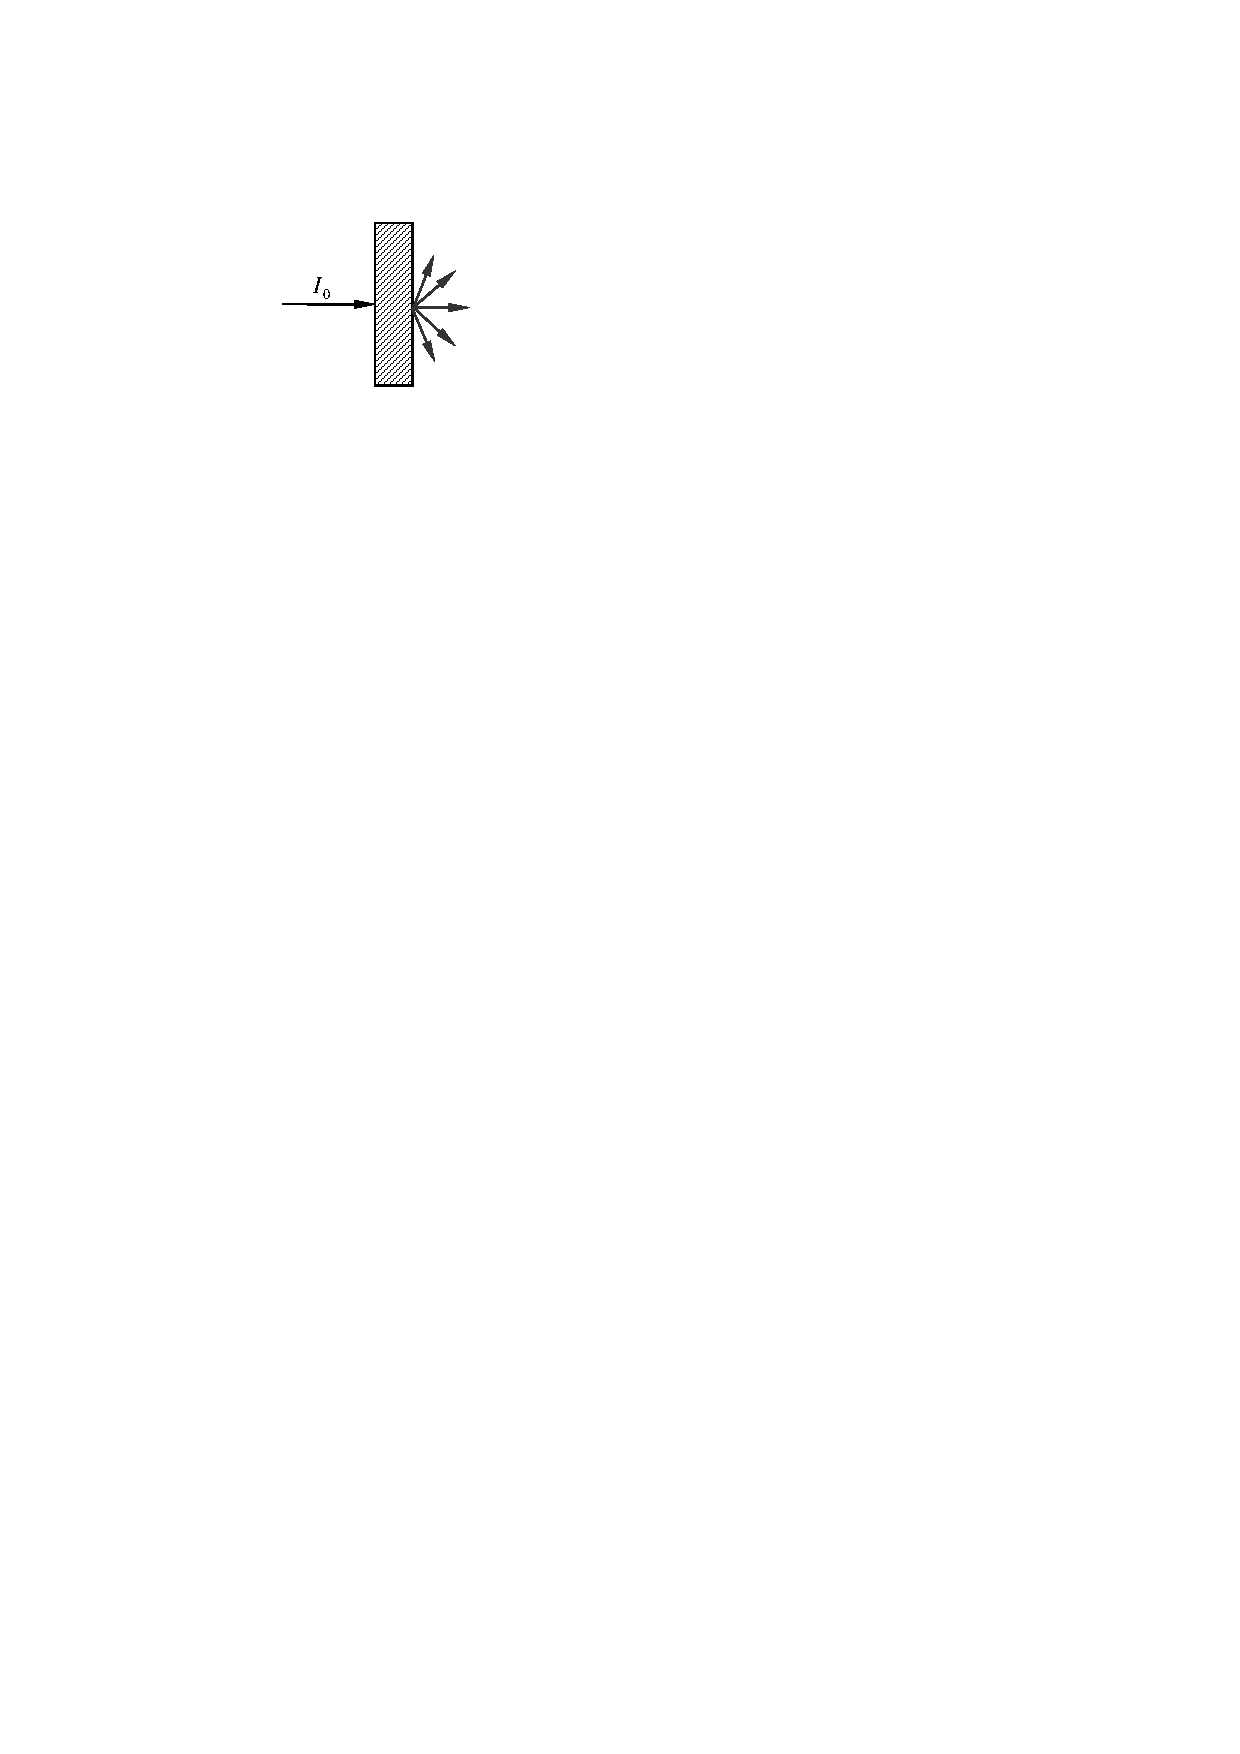
\includegraphics[width=0.5\textwidth]{fig12.pdf}
\caption{\label{fig12}粒子穿过材料}
\end{minipage}%
\begin{minipage}[b]{0.48\textwidth}
\centering
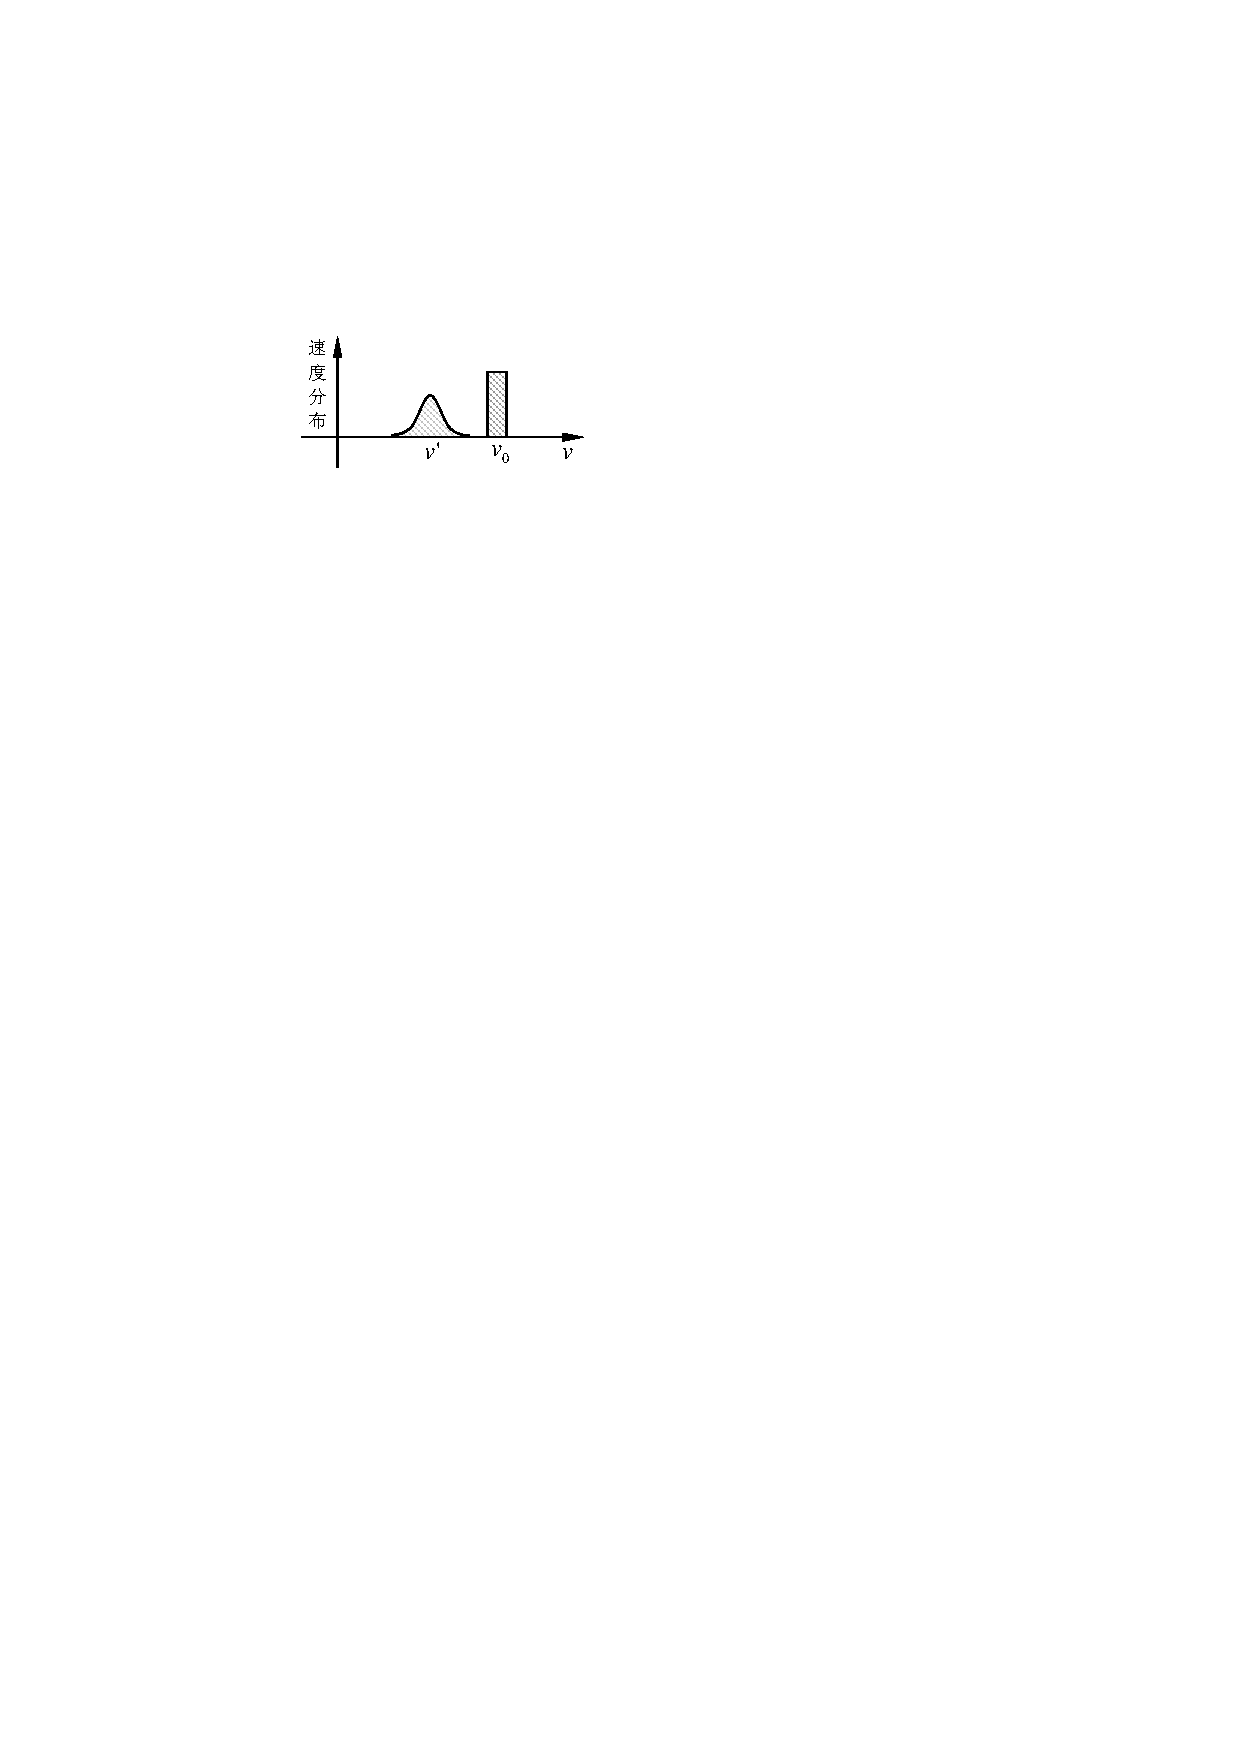
\includegraphics[width=0.6\textwidth]{fig13.pdf}
\caption{\label{fig13}出速粒子的速度分布}
\end{minipage}
\end{figure}
一束粒子强度为$I_0$, 通过厚度为$\textrm{d}x$的吸收体后, 强度必然减少, 减少量$\textrm{d}I$显然正比于厚度$\textrm{d}x$, 也正比于束流的强度$I$, 若把比例常数记为$\mu$, 则有
\[
-\textrm{d}I=\mu I(x)\textrm{d}x
\]
积分后得到
\[
I=I_0e^{-\mu x}
\]
这就是朗伯-比耳(Lambert-Beer)定律, 它不仅适用于粒子, 也适用于波(当然, 用于波时, 图\ref{fig13}将不再表示波的速度, 而表示波的频率). 

\noindent[\textbf{思考}]: 对于速度分布为图\ref{fig13}出射粒子, 其德布罗意波长分布是怎样的?电子的衍射实验能证明衍射图案是电子直接产生的吗, 能证明粒子的波动性吗, 为什么?

\subsection{康普顿(Compton)散射}
\begin{figure}[!htb]
\centering
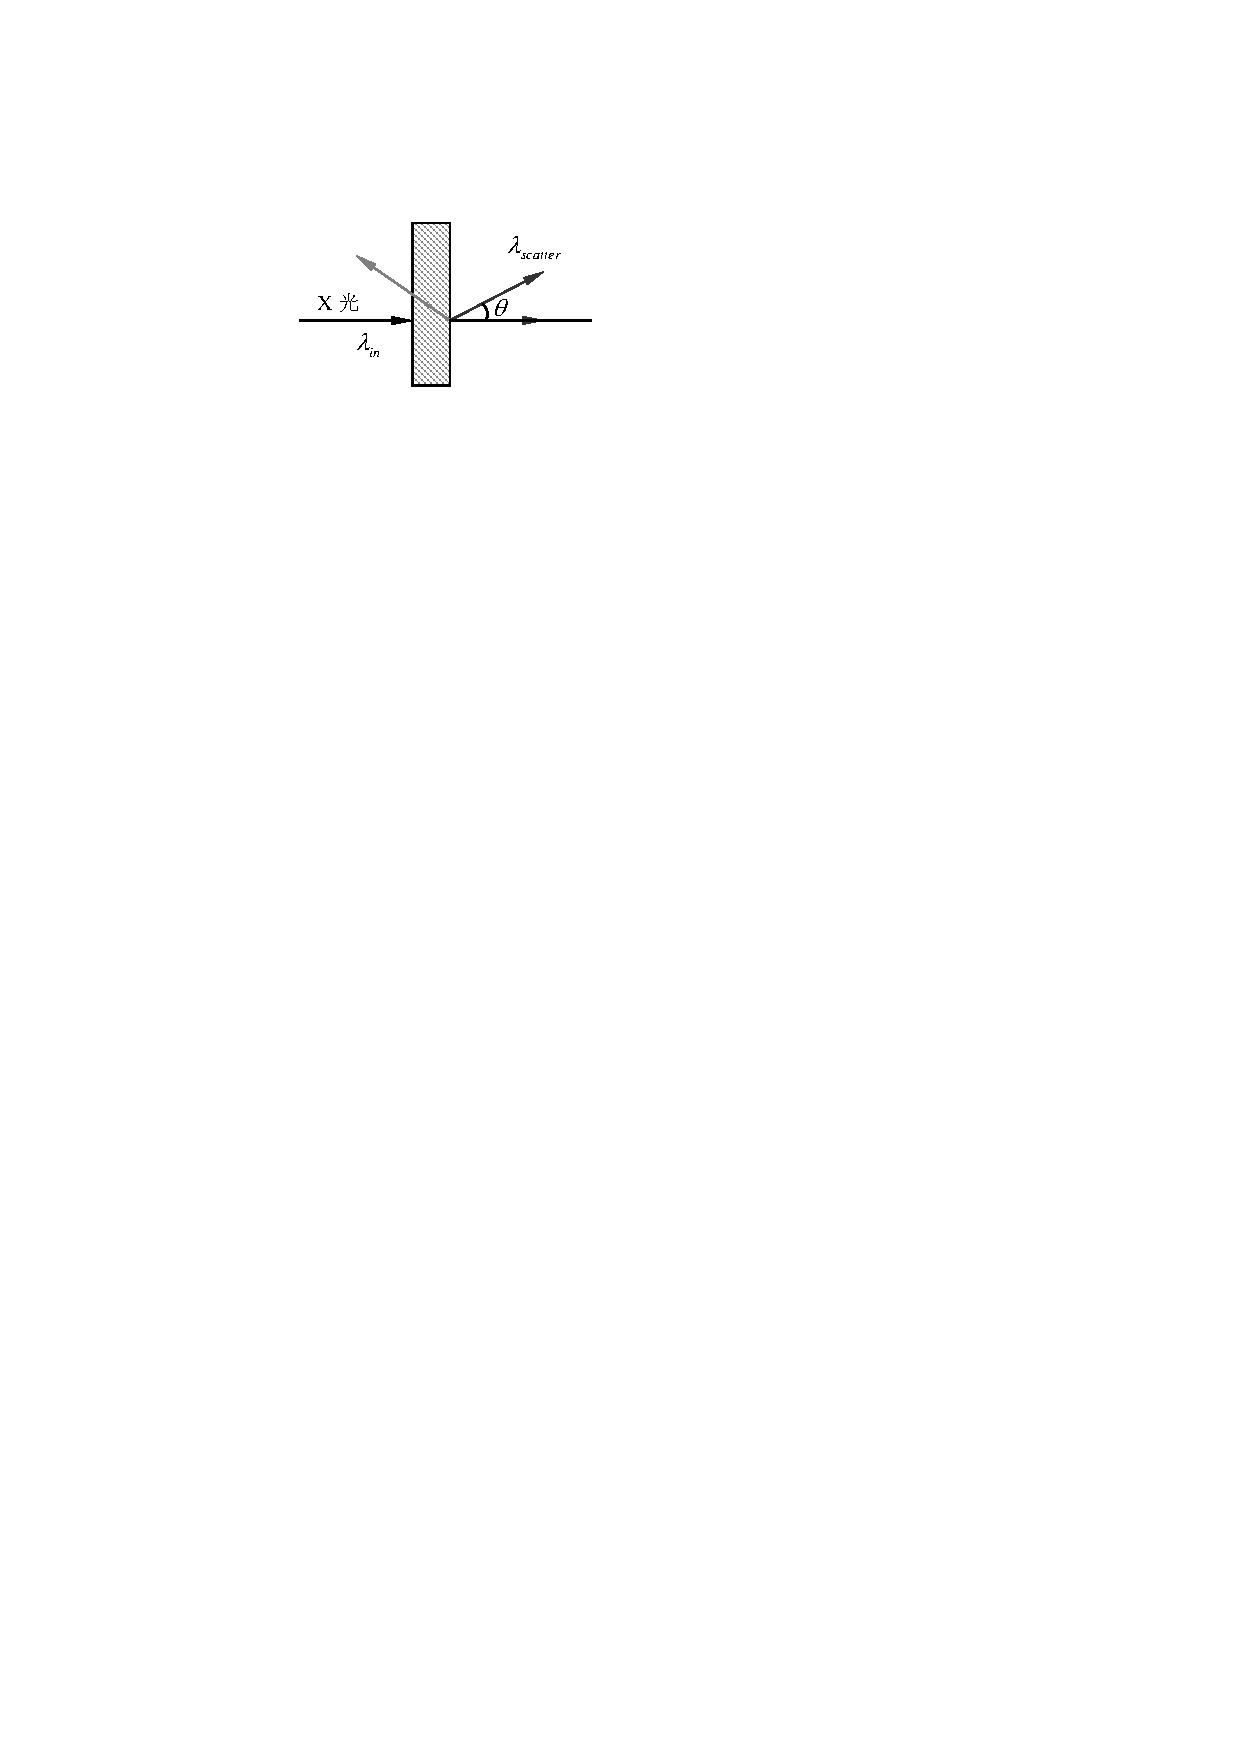
\includegraphics[width=0.35\textwidth]{fig11.pdf}
\caption{\label{fig11}康普顿散射}
\end{figure}
用X光照射晶体材料, 入射$\lambda_{in}$与出射$\lambda_{Scatter}$有以下关系: 
\[
\Delta\lambda=\lambda_{scatter}-\lambda_{in}=2k\sin^2\frac{\theta}{2}
\]
$k$是常数, 实验测得. 当换材料时, 公式不变, 即散射结果与材料无关. 揭示: 反映原子外层电子信息. 

\subsection{其它散射}
\begin{itemize}
\item \textbf{锐利散射}: 入射光在线度小于光波长的微粒上散射后散射光和入射光波长相同. 
\[
I_{sc}\propto\frac{k}{\lambda^4}
\]
正午时, 太阳直射地球表面, 太阳光在穿过大气层时, 各种波长的光都要受到空气的散射, 其中波长较长的波散射较小, 大部分传播到地面上. 而波长较短的蓝, 紫光, 受到空气散射较强, 但是人对紫光不敏感. 天空中的蓝色正是这些散射光的颜色, 因此天空会呈现蓝色. 
\begin{figure}[!htb]
\centering
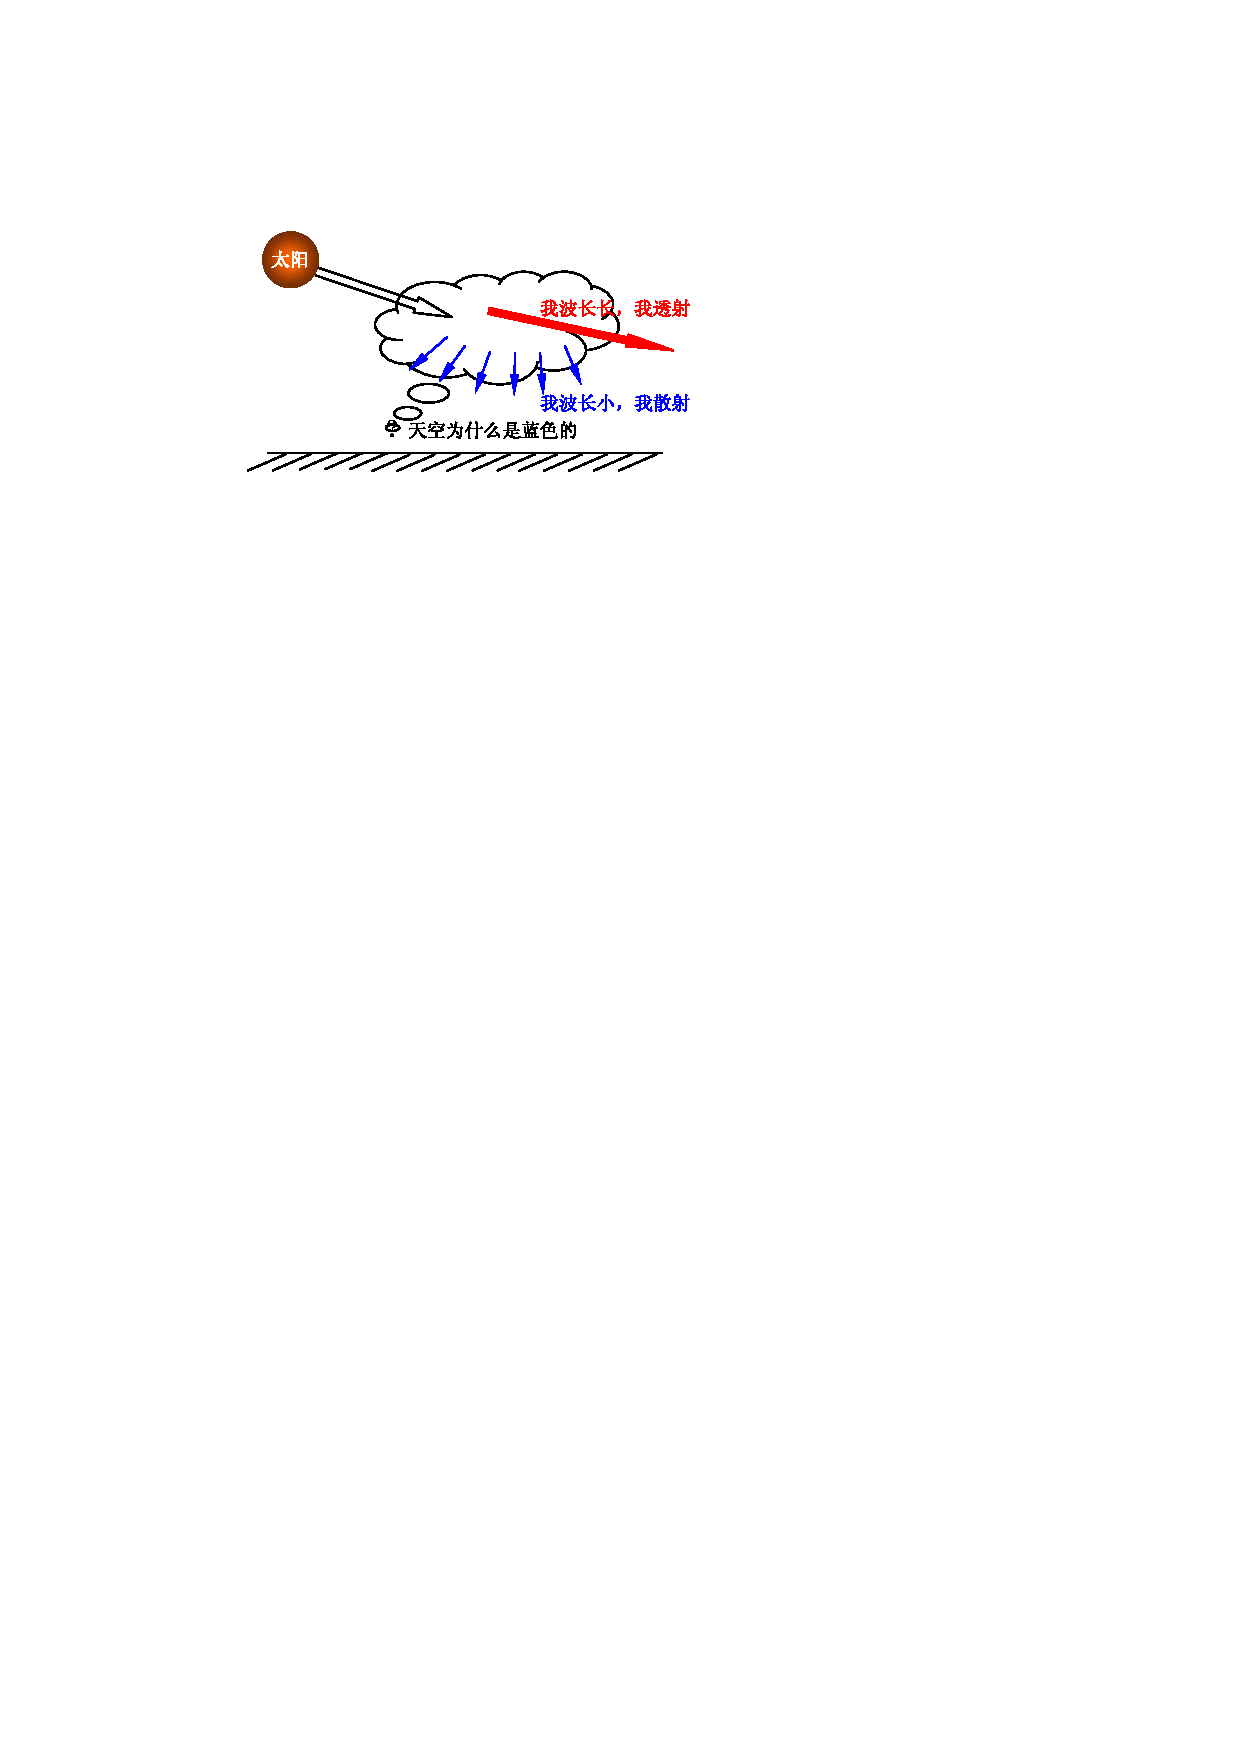
\includegraphics[width=0.5\textwidth]{fig17.pdf}
\caption{天空为什么是蓝色?}
\end{figure}

\item \textbf{拉曼散射}: 光通过介质时由于入射光与分子运动相互作用而引起的频率发生变化的散射.  拉曼散射也有$\Delta\lambda=\lambda_{sctter}-\lambda_{in}$, 但没有康普顿散射. 拉曼散射一般用紫外光, 而紫外光尺度大于原子, 只能反应分子的相互作用信息. 
\end{itemize}



\newpage
\section{原子核物理概论}
\subsection{三种射线的性质}
\begin{enumerate}
\item $\alpha$: He核束. 电离能力最强, 穿透能力最弱. 
\item $\beta$: 电子束. 
\item $\gamma$: 频率极高(高于X光)的电磁波. 穿透能力最强, 电离能力最弱. 
\end{enumerate}
$\alpha$, $\beta$, $\gamma$三种射线电离性依次减弱, 穿透性依次增强. 

\subsection{裂变和聚变}
\begin{itemize}
\item \textbf{裂变}: 用慢中子(为什么要用慢中子?)轰击轴235的反应式(下式只是其中一种形式, 还有其它的裂变方式)
\[
\textrm{n}+^{235}\textrm{U}\longrightarrow^{236}\textrm{U}^*\longrightarrow^{144}\textrm{Ba}+^{89}\textrm{Kr}+3\textrm{n}
\]
美国在日本广岛和长崎爆炸的两颗原子弹分别以$^{235}\textrm{U}$和$^{239}\textrm{Pu}$为燃料. 
$^{235}\textrm{U}$只占天然铀0.72\%, $^{238}\textrm{U}$占天然铀99.27\%, 
虽然$^{238}\textrm{U}$不能直接应用, 却可以用它来生产有用的核燃料, 下式是$^{238}\textrm{U}$反应制$^{239}\textrm{Pu}$
\[
\textrm{n}+^{238}\longrightarrow^{239}\textrm{U}+\gamma
\]
\[
^{239}\textrm{U}\longrightarrow^{239}\textrm{Np}+\textrm{e}^-+\overline{\nu}_e
\]
\[
^{239}\textrm{Np}\longrightarrow^{239}\textrm{Pu}+\textrm{e}^-+\overline{\nu}_e
\]
\item \textbf{聚变}: 氢弹的反应属于轻核聚变, 能放出巨大的能下, 反应式
\[
\textrm{d}+\textrm{T}\longrightarrow\alpha+\textrm{n}+17.58\textrm{MeV}
\]
氘(d)在自然界很长见, 但氚(T)在自然界中却不存在, 但可能通过下式反应制得
\[
\textrm{n}+^6\textrm{Li}\longrightarrow\alpha+\textrm{T}+4.9\textrm{MeV}
\]
\end{itemize}



\newpage
\begin{thebibliography}{10}
\bibitem{1} 罗骥老师2008学年上半学期的原子物理学授课内容。
\bibitem{2} 杨帅的原子物理学参考习题。
\bibitem{3} Stern-Gerlach experiment\\http://en.wikipedia.org/wiki/Stern\%E2\%80\%93Gerlach\_experiment
\bibitem{4} Zeeman-effect \\http://en.wikipedia.org/wiki/Zeeman\_effect
\bibitem{5} 斯塔克效应 \\http://www.wiki.cn/wiki/\%E6\%96\%AF\%E5\%A1\%94\%E5\%85\%8B\%E6\%95\%88\%E5\%BA\%94
\bibitem{6} 瑞利散射 \\http://baike.baidu.com/view/421229.html
\bibitem{7} 某同学原子物理学课堂笔记。
\bibitem{8} 杨福家,原子物理学(第三版),高等教育出版社。1999.5
\end{thebibliography}


\newpage
\appendix
\appendixpage

\begin{center}
{\Large 参考习题}
\end{center}

\begin{enumerate}
\item 简答
\begin{enumerate}
\item 给出德布罗波公式及推导, 并简述其合理性. 
\item 给出光电效应的能量关系公式, 并简述电位不同时,电子溢出情况是否满足光电效应的能量关系公式, 为什么?
\item 金和铂的区分方法. 
\item 什么是泡利不相同原理?意义:多电子原子,每个电子与原子关系能否相同.
\item 氢原子几何结构模型. 
\item 什么实验引出密里根射线, 阴极射线, $\alpha$粒子散射, $\alpha$粒子天然放射性.
\end{enumerate}

\item 推导计算
\begin{enumerate}
\item 朗泊-比耳定理
\item 卢瑟福公式(散射.图形.关系)
\item 库仑定律
\end{enumerate}

\item 分析论述
\begin{enumerate}
\item 拉曼, 康普顿散射与原子关系,条件. 
\item 弗朗赫兹实验(装置,光谱,汞蒸气,氩气), 吸收的能量. 
\item 斯坦克, 塞曼效应:条件及结果. 
\item 斯特恩-盖拉赫条件, 结果. 
\item 原子弹的工作原理, 核素的提取. 
\end{enumerate}

\end{enumerate}

\end{document}

